\documentclass[11pt,a4paper]{report}

% ============================================================
% EDITABLE DETAILS
% ============================================================
\newcommand{\StudentName}{Dulhara Anjana Langappuli}
\newcommand{\ShortStudentName}{Dulhara Langappuli}
\newcommand{\StudentNumber}{22044421}
\newcommand{\SupervisorName}{Professor Saeid Gorgin}
\newcommand{\AcademicYear}{2025-26}
\newcommand{\LevelName}{Level 7}
\newcommand{\SchoolName}{School of Physics, Engineering and Computer Science}
\newcommand{\DegreeName}{MSc Computer Science}
\newcommand{\ProgrammeName}{Artificial Intelligence and Robotics}
\newcommand{\ModuleName}{MSc CS Project}
\newcommand{\ReportName}{Final Project Report}
\newcommand{\ShortReportName}{FPR}
\newcommand{\ProjectTitle}{FPGA-Based Driver Distraction Detection System Using Image Classification}
\newcommand{\ShortProjectTitle}{Driver Distraction Detection System}
\newcommand{\SubmissionDate}{\today}

% ============================================================
% FONT, LANGUAGE AND PAGE LAYOUT
% ============================================================
\usepackage[british]{babel}
\usepackage[T1]{fontenc}
\usepackage[utf8]{inputenc}
\usepackage{lmodern}
\usepackage[a4paper,margin=2.5cm]{geometry}
\usepackage{microtype}
\usepackage{setspace}

\setstretch{1.15}
\setlength{\emergencystretch}{3em}

% ============================================================
% FIGURES AND TABLES
% ============================================================
\usepackage{graphicx}
\graphicspath{{images/}}

\usepackage{float}
\usepackage[section]{placeins}
\usepackage{caption}
\usepackage{subcaption}
\usepackage{array}
\usepackage{tabularx}
\usepackage{longtable}
\usepackage{booktabs}

% ============================================================
% CODE LISTINGS
% ============================================================
\usepackage{listings}
\usepackage{xcolor}

\definecolor{codegreen}{rgb}{0.0, 0.45, 0.0}
\definecolor{codeblue}{rgb}{0.0, 0.0, 0.85}
\definecolor{codered}{rgb}{0.6, 0.1, 0.1}
\definecolor{codegray}{rgb}{0.5, 0.5, 0.5}
\definecolor{codebg}{rgb}{0.97, 0.97, 0.97}

\lstset{
  basicstyle=\ttfamily\footnotesize,
  breaklines=true,
  frame=single,
  numbers=left,
  numberstyle=\tiny\color{codegray},
  columns=fullflexible,
  keywordstyle=\color{codeblue}\bfseries,
  commentstyle=\color{codegreen}\itshape,
  stringstyle=\color{codered},
  backgroundcolor=\color{codebg},
  captionpos=b
}

\newcolumntype{Y}{>{\raggedright\arraybackslash}X}

% ============================================================
% FIGURE COMMANDS
% ============================================================

% A required figure displays a placeholder when the file is missing.
\newcommand{\RequiredFigure}[4][0.88\textwidth]{%
  \begin{figure}[htbp]
    \centering
    \IfFileExists{images/#2}{%
      \includegraphics[width=#1]{#2}%
    }{%
      \fbox{%
        \parbox[c][4.1cm][c]{0.82\textwidth}{%
          \centering
          \textbf{Missing figure}\par
          Upload \texttt{\detokenize{#2}} to the
          \texttt{images} folder.
        }%
      }%
    }
    \caption{#3}
    \label{#4}
  \end{figure}
}

% Allow LaTeX to place figures more efficiently.
\setcounter{topnumber}{3}
\setcounter{bottomnumber}{2}
\setcounter{totalnumber}{5}

\renewcommand{\topfraction}{0.90}
\renewcommand{\bottomfraction}{0.80}
\renewcommand{\textfraction}{0.08}
\renewcommand{\floatpagefraction}{0.75}

% Put figures at the top of figure-only pages.
\makeatletter
\setlength{\@fptop}{0pt}
\setlength{\@fpsep}{12pt plus 2pt minus 2pt}
\setlength{\@fpbot}{0pt plus 1fil}
\makeatother

% A large and readable figure command.
\newcommand{\ReadableFigure}[4][0.92\textwidth]{%
  \begin{figure}[!htbp]
    \centering
    \IfFileExists{images/#2}{%
      \includegraphics[
        width=#1,
        height=0.70\textheight,
        keepaspectratio
      ]{images/#2}%
    }{%
      \fbox{%
        \parbox[c][5cm][c]{0.85\textwidth}{%
          \centering
          \textbf{Missing figure}\\
          \texttt{\detokenize{#2}}
        }%
      }%
    }
    \caption{#3}
    \label{#4}
  \end{figure}
}

% An optional figure is omitted when its file is absent.
\newcommand{\OptionalFigure}[4][0.88\textwidth]{%
  \IfFileExists{images/#2}{%
    \begin{figure}[htbp]
      \centering
      \includegraphics[width=#1]{#2}
      \caption{#3}
      \label{#4}
    \end{figure}
  }{}
}

\usepackage{enumitem}

% ============================================================
% LINKS AND HARVARD REFERENCES
% ============================================================
\usepackage{csquotes}
\usepackage{url}
\usepackage[authoryear,round]{natbib}

\bibpunct{(}{)}{;}{a}{,}{,}

\usepackage{hyperref}

\hypersetup{
  colorlinks=true,
  linkcolor=black,
  citecolor=black,
  urlcolor=blue,
  pdftitle={\ReportName\ - \ProjectTitle},
  pdfauthor={\StudentName},
  pdfsubject={MSc Project Final Project Report}
}

\urlstyle{same}

% ============================================================
% DOCUMENT
% ============================================================
\begin{document}

\raggedbottom

% ============================================================
% TITLE AND DECLARATION
% ============================================================
\pagenumbering{gobble}
\pagestyle{empty}

%!TEX root = main.tex
\begin{titlepage}
\thispagestyle{empty}
\begin{center}
  \IfFileExists{images/UH_logo.PNG}{%
    
\includegraphics[width=0.32\textwidth]{UH_logo.PNG}%
  }{%
    \fbox{\parbox[c][2.0cm][c]{0.60\textwidth}{\centering Upload \texttt{UH\_logo.PNG} to the images folder.}}
  }

  \vspace{0.45cm}
  {\Large\bfseries \SchoolName\par}
  \vspace{0.08cm}
  {\Large\bfseries \DegreeName\par}
  \vspace{0.08cm}
  {\Large\bfseries \ProgrammeName\par}

  \vspace{0.80cm}
  {\large Module: \ModuleName\par}
  \vspace{0.15cm}
  {\LARGE\bfseries \ReportName\par}

  \vspace{0.72cm}
  {\LARGE\bfseries \ProjectTitle\par}

  \vspace{0.62cm}
  \IfFileExists{images/state_farm_sample_images.png}{%
    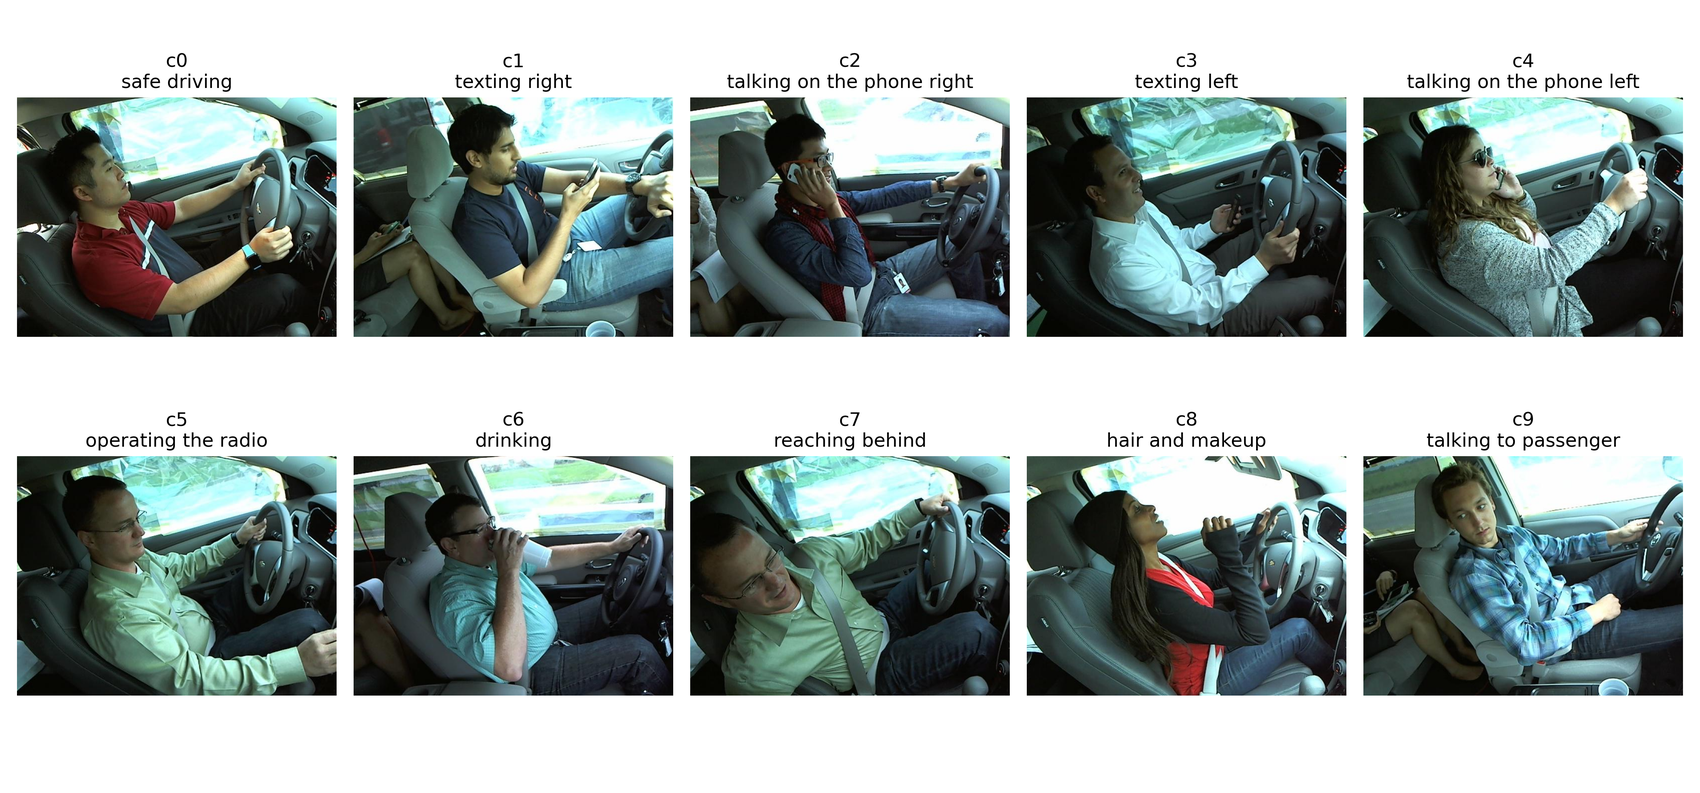
\includegraphics[width=0.78\textwidth,height=6.2cm,keepaspectratio]{state_farm_sample_images.png}%
  }{%
    \fbox{\parbox[c][5.6cm][c]{0.79\textwidth}{\centering Add a representative sample image to the images folder.}}
  }
\end{center}

\vfill
\begin{center}
\begin{tabular}{@{}l c l@{}}
Name & : & \StudentName \\[0.16cm]
Student ID & : & \StudentNumber \\[0.16cm]
Level & : & \LevelName \\[0.16cm]
Academic Year & : & \AcademicYear \\[0.16cm]
Supervisor & : & \SupervisorName
\end{tabular}
\end{center}

\vspace{0.9cm}
\begin{center}
\parbox{0.85\textwidth}{\small\centering
I confirm that this report has been critically proof-read and quality checked by me, and that it is free from grammar, spelling and formatting errors to the best of my knowledge, meeting the standards of clarity, coherence and presentation expected of this submission.
}
\end{center}
\vfill
\end{titlepage}

%!TEX root = main.tex

\thispagestyle{empty}

\begin{center}
  {\Large\bfseries Declaration}
\end{center}

\vspace{1cm}

\noindent
This report is submitted in partial fulfilment of the requirement for
the degree of Master of Science in Computer Science
(Artificial Intelligence and Robotics) at the University of
Hertfordshire.

\vspace{0.7cm}

\noindent
I hereby declare that the work presented in this project and report is
entirely my own, except where explicitly stated otherwise. All sources
of information and ideas, whether quoted directly or paraphrased, have
been properly referenced in accordance with academic standards. I
understand that any failure to properly acknowledge the work of others
could constitute plagiarism and may result in academic penalties.

\vspace{0.5cm}

\noindent
I did not use human participants in my MSc Project.

\vspace{0.5cm}

\noindent
I hereby \textbf{give} permission for the report to be made available
on the university website provided the source is acknowledged.

\vspace{1.2cm}

\noindent
\begin{tabular}{@{}l l@{}}
Signature: &
\IfFileExists{images/my_signature.png}{%
  \raisebox{-0.25\height}{%
    \includegraphics[
      width=8.2cm,
      height=3.0cm,
      keepaspectratio
    ]{images/my_signature.png}%
  }%
}{%
  \rule{4.2cm}{0.4pt}%
}
\\[0.45cm]

Name: & \StudentName \\[0.18cm]
Student ID: & \StudentNumber \\[0.18cm]
Date: & \SubmissionDate
\end{tabular}

\newpage

% ============================================================
% FRONT MATTER - ROMAN PAGE NUMBERS
% ============================================================
\clearpage
\pagenumbering{roman}
\setcounter{page}{1}
\pagestyle{plain}

\setcounter{tocdepth}{2}
\tableofcontents

\clearpage
\listoffigures

\clearpage
\listoftables

\clearpage
%!TEX root = main.tex

\chapter*{List of Abbreviations}
\addcontentsline{toc}{chapter}{List of Abbreviations}

\renewcommand{\arraystretch}{1.25}

\begin{longtable}{@{}p{0.18\textwidth}p{0.74\textwidth}@{}}
\toprule
\textbf{Abbreviation} & \textbf{Meaning} \\
\midrule
\endfirsthead

\toprule
\textbf{Abbreviation} & \textbf{Meaning} \\
\midrule
\endhead

AI       & Artificial Intelligence \\
ARM      & Processor architecture used by the ZC702's Cortex-A9 cores \\
AXI      & Advanced eXtensible Interface \\
BRAM     & Block Random-Access Memory \\
CNN      & Convolutional Neural Network \\
CPU      & Central Processing Unit \\
DSP      & Digital Signal Processing \\
F1       & Harmonic mean of precision and recall \\
FPGA     & Field-Programmable Gate Array \\
FPS      & Frames per second \\
GPIO     & General-Purpose Input/Output \\
INT8     & Eight-bit integer representation used for model quantisation \\
IR       & Infrared \\
LUT      & Lookup Table \\
NIR      & Near-Infrared \\
NoIR     & Camera without an infrared-blocking filter \\
PRISMA   & Preferred Reporting Items for Systematic Reviews and Meta-Analyses \\
RGB      & Red, Green and Blue colour representation \\
RTL      & Register-Transfer Level \\
SoC      & System-on-Chip \\
TFLite   & TensorFlow Lite \\
UART     & Universal Asynchronous Receiver-Transmitter \\
USB      & Universal Serial Bus \\
VFP      & Vector Floating Point \\
WNS      & Worst Negative Slack \\
XNNPACK  & Optimised neural-network inference library used by TensorFlow Lite \\

\bottomrule
\end{longtable}

\renewcommand{\arraystretch}{1}

% ============================================================
% MAIN CONTENT - ARABIC PAGE NUMBERS
% ============================================================
\clearpage
\pagenumbering{arabic}
\setcounter{page}{1}
\pagestyle{plain}

% ============================================================
% ABSTRACT
% ============================================================
%!TEX root = main.tex
\chapter*{Abstract}
\addcontentsline{toc}{chapter}{Abstract}

Most published driver-distraction detection systems are trained and tested on images from one fixed camera position, in daylight, with speed usually measured only on a laptop, not real hardware. This project asks what happens when each of those three assumptions is removed, and answers each one with real measurements instead of estimates.

Three CNN architectures, a custom CNN, MobileNetV2 and EfficientNet-B0, were trained on the State Farm Distracted Driver Detection dataset. The training used a subject-wise split that holds entire drivers out of training, which avoids the subject leakage caused by a random image-level split. MobileNetV2 was chosen as the best model, with 84.67\% test accuracy and 84.01\% macro F1. Two robustness tests were then run on real data. For camera view, State Farm was combined with the SAM-DD multi-view dataset, and a frozen-backbone model reached only 75.94\% mixed-view accuracy, uneven across views, and fine-tuning raised this to 91.76\%. For lighting, the day-trained model was tested on real night footage recorded under active infrared light, replacing an earlier plan to make synthetic infrared-like images, since a synthetic transform can only approximate real infrared data, not replace it. The model's accuracy collapsed to 19.53\%, with zero recall on eight of the ten classes. Training on real night data brought night accuracy back up to 71.13\%, at a cost of 3.5 points of daytime accuracy.

The fine-tuned model was quantised to INT8 TensorFlow Lite, reducing its size 8.00$\times$, from 20.78~MB to 2.60~MB, for a cost of 2.7 accuracy points. It was then deployed on a Xilinx ZC702 board, after fixing a CPU instruction-set mismatch in the only published runtime for that platform. On-device accuracy was 77.3\%, with 100 out of 100 prediction agreement against the reference model. Inference took about 9.15 seconds per image, roughly 150$\times$ slower than the laptop figure and the clearest limitation of this deployment. A separate FPGA alert-decision stage was verified in simulation against real model predictions, including real misclassifications, and synthesised to 18 LUTs and 13 flip-flops, with 7.276~ns of positive timing slack.

The results show three things. First, camera-view and lighting robustness have to be trained for on purpose, they do not happen by themselves. Second, the cost of embedded deployment falls almost entirely on the classifier and not on the logic around it. Third, measuring a robustness problem before fixing it is what makes the fix easy to understand.


% ============================================================
% MAIN CHAPTERS
% ============================================================
%!TEX root = main.tex

\chapter{Introduction}
\label{ch:introduction}

\section{Problem overview}

Distracted driving is a major road-safety problem. Activities such as using a phone, eating, drinking, adjusting vehicle controls or talking to a passenger can take a driver's attention away from the road. Camera-based classification offers a practical way to recognise these behaviours and generate an alert when sustained distraction is detected.

The difficulty is that many published systems are developed and evaluated under controlled conditions, usually with one camera position and one lighting condition. Strong accuracy under those conditions does not guarantee comparable performance from another viewpoint or at night. A usable in-car system must also run on suitable hardware and turn individual frame predictions into stable alerts. This project examines these modelling and deployment problems as parts of the same system.

\section{Current issues and the gap this project addresses}

Three gaps motivate this project. Chapter~\ref{ch:litreview} assesses each gap against the existing literature.

First, camera-view robustness is rarely tested directly. In data where multi-view options exist, much previous research either uses a single view or measures performance inside a viewpoint rather than across viewpoints. The existence of left and right distraction classes further complicates this problem because a frontal camera provides a mirrored view in relation to the side camera view and thus "texting left" performed with the former will look like "texting right" when captured with the latter. Pooling across views without addressing this discrepancy runs the risk of quietly skewing labels.

Second, while lighting robustness is a widely recognized problem, its evaluation is rarely conducted with actual data. Where low-lighting scenarios are included in evaluations, researchers frequently use artificially dimmed daytime images or infrared-like coloring, which is a perfectly acceptable proxy for robustness but is no replacement for real low-light images. Real low-light data captures effects that cannot be created synthetically, such as color attenuation, the impact of near infrared illumination on skin and fabric reflections and camera noise. This project initially considered doing a synthetic experiment of this sort but abandoned it in favor of real low-light data once it became available.

Third, the progression from a trained model to a functioning alert system is generally seen as a promising future development rather than something to be actually implemented. Frames per second measurements are usually obtained using development workstation scale benchmarks rather than on realistic hardware configurations. Quantization effects on accuracy and model size are rarely considered and the process used to transform frame-wise predictions into an alert is even more rarely explained and validated empirically.

\section{Project details}

The project is built in two connected phases that match these gaps.

\textbf{Phase 1 - AI robustness.} A single-view baseline is set up first. Custom CNN, MobileNetV2 and EfficientNet-B0 are trained on the State Farm Distracted Driver Detection dataset (10 classes, 22{,}424 images) using a subject-wise split. These three models are then tested and compared in terms of accuracy, macro F1, per class recall and throughput. Next, two robustness tests are run on real data. First, camera-view robustness test consists of combining State Farm (side view) and SAM-DD dataset, which contains images in pairs from front- and side-views. Second, lighting robustness is tested by combining State Farm and nighttime subset of the Low-Light Driver Distraction Dataset \citep{saad2020lowlight}, recorded in active infrared light. This test evaluates the drop in accuracy of day-only model before any intervention is taken.

\textbf{Phase 2 - hardware.} The fine-tuned model is converted into quantized INT8 TensorFlow Lite format and deployed on the Xilinx ZC702 board (Zynq-7000) for the reason that this board contains a general-purpose CPU ARM Cortex-A9 core that can perform a full CNN, unlike an FPGA board without a core on board. Real latency and accuracy is measured instead of being estimated. Decision stage with hysteresis logic in order to prevent flickering alerts is implemented in Verilog, verified through simulation by comparing the decision stage predictions to the predictions made by the trained model. Finally, the alert pathway from the board to a backend and Android client is set up.

\section{Aims and objectives}

\begin{enumerate}[itemsep=0.15em]
	\item To prepare and use suitable driver-distraction image data, including real multi-view and real low-light data, for training and testing a camera-view-robust and lighting-robust classification system.
	\item To build and test a prototype running on real, low-cost embedded hardware, with an alert output that reacts to sustained distraction rather than a single momentary prediction and to measure the accuracy, size and latency cost of getting there.
\end{enumerate}

\section{Research questions}
\label{sec:research-questions}

\begin{enumerate}[itemsep=0.15em]
	\item[\textbf{RQ1}] How do a custom CNN, MobileNetV2 and EfficientNet-B0 compare when the test drivers are not present in the training data?
	\item[\textbf{RQ2}] How much does accuracy change when a model is tested on a different, unseen camera view and does fine-tuning on multi-view data close that gap?
	\item[\textbf{RQ3}] How much accuracy does a day-trained model lose on real infrared-illuminated footage and how much can be recovered by training on real night data rather than synthetic approximations?
	\item[\textbf{RQ4}] What does INT8 quantisation and embedded deployment cost in accuracy, model size and latency before and after conversion and how do laptop figures differ from real on-device performance?
	\item[\textbf{RQ5}] Which part of a complete pipeline, the classifier or the decision logic after it, can actually be built and checked in FPGA hardware in the time available?
\end{enumerate}

Every experiment in Chapter~\ref{ch:results} is tied to one of these questions. Section~\ref{sec:qr-rq-summary} gives the answer each one produced.

\section{Feasibility, commercial context and risk}

The scope has been defined to include aspects which could be physically implemented and measured, as opposed to purely simulated. A fully functional CNN accelerator based on an FPGA was seen to be too challenging for the timeline and was thus discarded. The ZC702’s Cortex-A9 core runs the classifier and the fabric is used for the decision making stage. This solution was known in advance to be a fall-back plan from the very start from the Interim Progress Report.

The business case of the project is based on cost, rather than novelty. As driver monitoring becomes mandatory for new cars of certain categories in several countries, current systems are developed by the manufacturers. However, in the retrofit and fleet sector, which is the target market, older cars, taxis, delivery vans, driving schools, et cetera are equipped with hardware of much more modest budget. That is why the project aims at using components costing in tens of pounds, as opposed to thousands. Among other risks are the possibility of drivers not taking kindly to surveillance, legal issues arising due to false alerts and the obvious gap between an experimental proof of concept and a commercially viable product, which is covered in more detail in Chapter~\ref{ch:evaluation}.

The key technical problem that emerged during the project was an incompatibility at the low level of the single existing TensorFlow Lite runtime for this board and the actual instruction set (Section~\ref{sec:arm32-issue}). Fixing this problem instead of giving up on local inference was one of the main technical contributions of the project.

\section{Report structure}

Chapter~\ref{ch:litreview} reviews prior work related to distraction detection, cross view and lighting robustness and embedded/FPGA-based deployment. Chapter~\ref{ch:methodology} covers data preparation, model training, quantisation, FPGA implementation, buzzer-overlay implementation and testing strategy. Chapter~\ref{ch:results} contains the results with critical analysis, including a software/hardware performance comparison. Chapter~\ref{ch:evaluation} evaluates the project according to its goals, literature review, project management, limitations and future work.

%!TEX root = main.tex

\chapter{Literature Review}
\label{ch:litreview}

\section{How the literature for this project was selected}
\label{sec:lit-prisma}

This review was based on a PRISMA-style search and screening exercise completed in June 2026 \citep{page2021prisma,prisma2020}. The search covered IEEE Xplore, Google Scholar, SpringerLink, MDPI, Elsevier, ScienceDirect, arXiv, dataset records and citation tracing. Search terms were organised around three parts of the project which are RGB driver-distraction classification, embedded deployment and lighting robustness.

The search identified 90 records, of which 22 were duplicates. Following title, abstract and full-text screening, 31 studies were retained: 20 core studies and 11 supporting studies. Figure~\ref{fig:prisma} summarises the process, while the complete search and exclusion details are provided in Appendix~\ref{app:prisma}.

\begin{figure}[htbp]
\centering
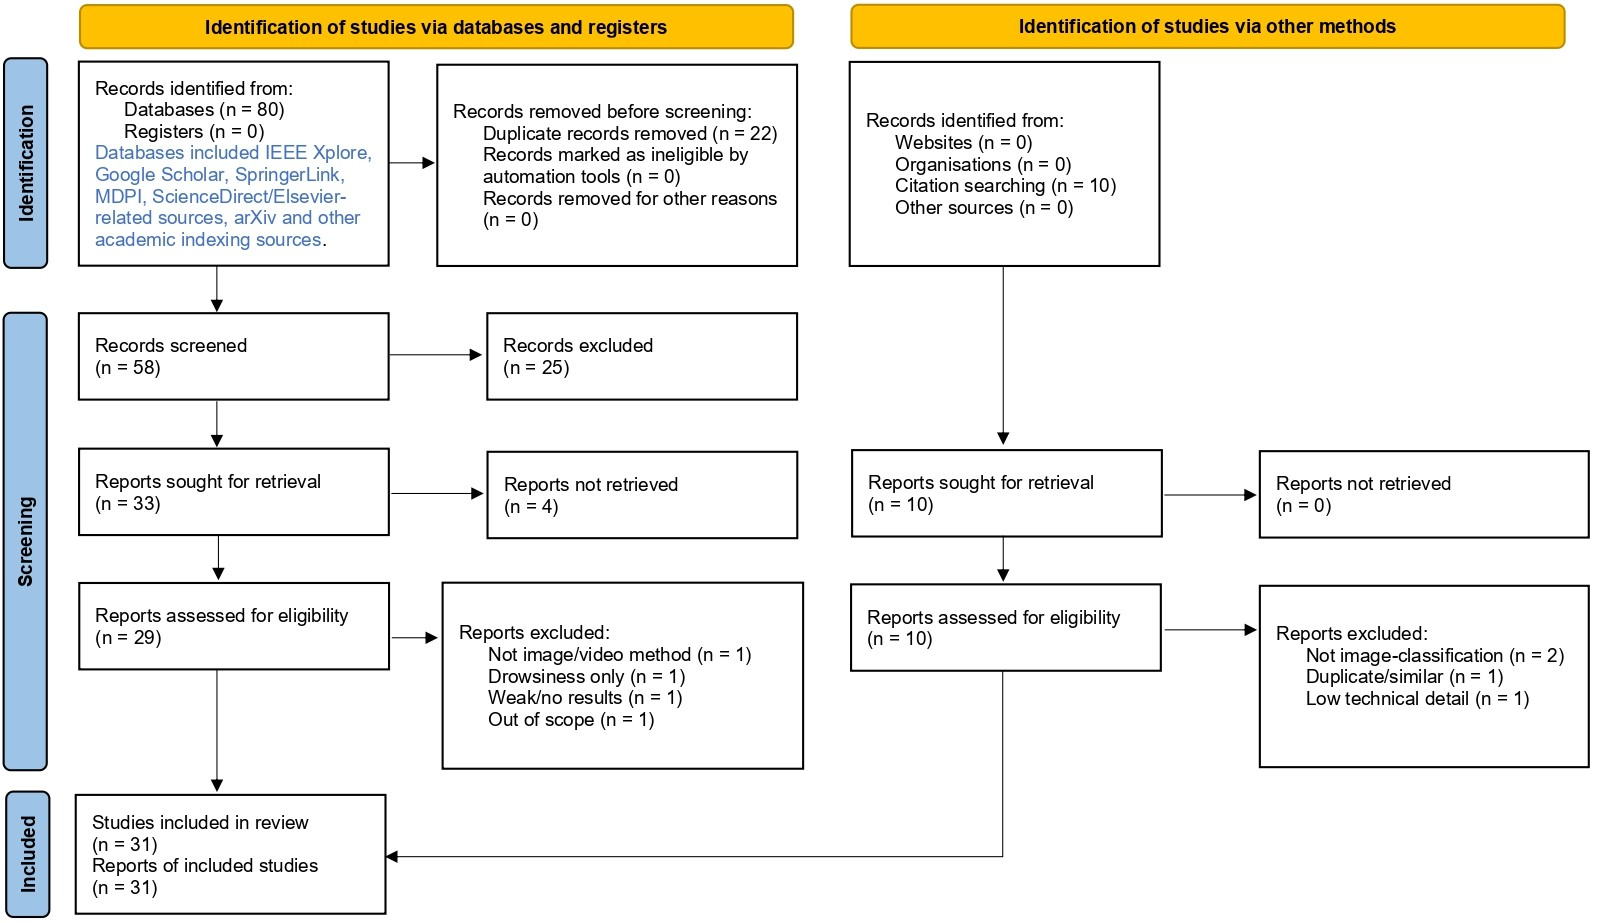
\includegraphics[width=1.0\textwidth]{fig_prisma_flow_diagram.png}
\caption{PRISMA-style selection process for the systematic search underpinning this review (90 records identified, 20 core studies selected).}
\label{fig:prisma}
\end{figure}

Two patterns from the review shaped this project. First, accuracy values from different studies are not directly comparable when their datasets and splitting protocols differ. For example, a high result from a random image-wise split may provide weaker evidence of generalisation than a lower result from a subject-wise split. Second, claims about embedded deployment are more common than measurements collected on the target device. These findings motivated the consistent use of subject-wise evaluation and the separation of laptop and on-device measurements in Chapter~\ref{ch:results}.

\ReadableFigure[0.96\textwidth]
{fig_reported_accuracy_comparison.png}
{Reported accuracy across the core studies. Differences reflect the datasets and evaluation protocols as well as model performance.}
{fig:reported-accuracy}

\ReadableFigure[0.96\textwidth]
{fig_deployment_maturity.png}
{Deployment maturity evidence across the selected studies. Measurements collected on embedded target devices are less common than offline evaluations.}
{fig:deployment-maturity}

\FloatBarrier

\section{Image-based driver distraction detection}

The application of CNNs for image-based distraction detection is a well-established topic. In particular, \citet{valeriano2018recognition} train a CNN on the State Farm dataset used in this research, demonstrating good within-view results and showing that ten classes taxonomy can be learned using only one side-mounted camera without any other sensors. \citet{alshalfan2021detecting} and \citet{aljasim2022e2dr} continue research in this direction. While the first paper evaluates several deep architectures on the same task, the second paper presents an ensemble technique that, once the distraction is detected, gives a recommendation as to how to respond to it, thus considering classification a part of the bigger decision-making process – an approach close to the one taken in this paper, where the decision stage after the classifier is carefully designed.

\citet{abouelnaga2018} and \citet{eraqi2019driver} have introduced AUC Distracted Driver dataset and an ensemble method using it, thus providing evidence that the State Farm taxonomy is transferable to an independently collected dataset. It has become the motivation behind the choice of AUC V2 during the multi-view stage, despite being unavailable at the time of this project. General reviews by \citet{kashevnik2021driver}, \citet{horgan2021} and \citet{dontoh2025visual} confirm the existence of the above pattern rather than provide just one example: the reported systems are mostly evaluated on a single camera position and under a certain lighting condition, which are seen as properties of the dataset rather than its variables to be tested.

MobileNetV2 and EfficientNet-B0 were selected as transfer-learning candidates because they offer different compromises between accuracy and computational cost. MobileNetV2 was designed for resource-constrained deployment \citep{sandler2018mobilenetv2}, while EfficientNet-B0 provides a compact benchmark based on balanced scaling of network depth, width and resolution \citep{tan2019efficientnet}.

\section{Subject-wise evaluation, dataset bias and domain shift}

The issue that repeatedly emerges in the context of this field and is handled in this work rigorously is subject leakage. If a driver appears in the training and test sets simultaneously, the split into training and testing samples randomly based on images overestimates the real-world accuracy of a model, as it is able to use the appearance features (clothing, body build, seat position, etc.) of the driver rather than his behavior and consecutive video frames make this effect even more pronounced. This becomes the main reason why numbers presented in this field cannot be easily compared between papers. Thus, the subject-wise protocol described in Section~\ref{sec:method-splits} is consistently used on all datasets and project stages. \citet{wang2023driver} address a different but similar problem of domain shift due to changes in the conditions of recordings and demonstrate a significant drop of performance in such case. This result is consistent with the ones presented here, although the magnitude of drop under the lighting shift in real conditions (Section~\ref{sec:qr-lowlight}) is significantly higher.

\section{Multi-view and cross-view driver monitoring}
\label{sec:lit-crossview}

The prevalence of evaluations based on single-view data is not due to the lack of multi-view data and techniques. \citet{jegham2019mdad} created the MDAD, a multi-view, multi-modal driver action dataset built off synchronized side and front cameras, akin to SAM-DD \citep{yang2024samdd} used in the current project, proving that synchronization-based generation of cross-view data is a known approach, not a specific feature of this work. \citet{ortega2020dmd} and \citet{wang2023hundreddriver} extend the approach to larger multi-modal datasets. A different approach is taken by \citet{sengar2023poseviNet}, who extract the pose data from each viewpoint and combine it with a vision transformer, thus showing that viewpoint-aware features may be a plausible alternative to the fine-tuning approach employed in this work.

Most relevantly, \citet{bhalla2025crossview} tackle the cross-view issue in a two-step process: they learn viewpoint-invariant features through contrastive learning across viewpoints and then adapt these features to different sensors without target labeling, obtaining significant improvements over the older baselines. This approach is far superior to the technique used in this work of fine-tuning of the last 30 layers of an already trained backbone network using pooled multi-view data. However, the comparison is telling because despite the relatively simple fine-tuning technique used in this work, it was still able to recover most of the accuracy losses from the evaluation of the frozen-backbone network in a cross-view setup (Section~\ref{sec:qr-crossview}). Therefore, fine-tuning of the model on real paired data is a reasonable middle-ground for a project of this type, although contrastive adaptation is a more principled approach.

One distinctive thing about this project compared to the surveyed literature is that it explicitly evaluates the cross-view gap in a frozen backbone "before" taking any steps to address it. Very few of the surveyed papers provide an equivalent "before" baseline, making it hard to judge the typical size of the raw gap for a MobileNetV2-class model and the degree to which the claimed improvements are due to the suggested method vs just having multi-view training data available.

\section{Low-light, infrared and near-infrared driver monitoring}
\label{sec:lit-lowlight}

Nighttime driver monitoring could be considered the most relevant application scenario for a driver monitoring system of this kind, yet it appears to be underrepresented in the RGB-based classification literature. The most directly relevant work is \citet{saad2020lowlight}, who created the Novel Driver Distraction Dataset with low-light support \citep{saad2020dataset}, specifically because the benchmark datasets of the time lacked nighttime data and this is the dataset used in the current project (Section~\ref{sec:method-lowlight-data}). \citet{janveja2020insight} position low-light driver state monitoring as an embedded systems problem rather than a modeling one.

Methodologically, the key work in this area is \citet{shen2023visible}. It proposes a way to solve both day and nighttime driver state classification using visible-to-infrared image translation, producing images looking like infrared ones. This paper exemplifies the strengths and weaknesses of the synthetic approach: it offers a way to augment a small pool of night training data but is explicitly presented as an approximation, not a substitute for the real deal. This particular distinction is crucial in the current project's context. The initial idea for the lighting stage of this project included the translation technique described in \citet{shen2023visible}. However, the intentional decision was made to abandon it once real low-light data was available, since a synthetic transformation cannot duplicate the effect that infrared illumination has on a scene, namely, the loss of color information, the way skin and fabric reflect near-infrared light and the noise in the image caused by the low-light operation of the camera. That is why Section~\ref{sec:qr-lowlight} relies on the real footage with infrared illumination and all conclusions about lighting robustness made in this report are about real footage, not an approximation.

\section{Quantisation and embedded/FPGA deployment}
\label{sec:lit-embedded}

Edge deployment introduces costs that model accuracy alone does not show. \citet{abushahla2025quantization} identify INT8 post-training quantisation as a common first step for reducing the storage and computational cost of edge-AI models. The accuracy reductions measured in this project, ranging from 0.8 to 4.6 percentage points across different samples, are consistent with the small but data-dependent losses discussed in that literature. \citet{hariharan2023edge} similarly examine the practical requirements of deploying AI-based driver-monitoring systems.

The FPGA literature shows the difference between running a model on an embedded processor and accelerating it in programmable logic. \citet{parra2023methodology} describe a custom AXI-Lite accelerator for a TensorFlow-Lite-quantised CNN on a Zynq device. More directly, \citet{lu2025hardware} implement a MobileNetV2-based driver-behaviour accelerator on the same XC7Z020 device family used here, achieving 13.05 FPS at 1.25 W.

Those systems are substantially more complex than the implementation in this project. Here, the classifier runs on the Cortex-A9 processor and the FPGA fabric handles only the alert-decision stage. This choice kept the work achievable within the project scope, but produced a much lower speed of approximately 9.15 seconds per inference. Reporting that limitation alongside the successful deployment gives a more realistic comparison with dedicated accelerators.

\section{Gaps identified and positioning of this project}

Figure \ref{fig:landscape} demonstrates how this project fits into the landscape of the surveyed literature, while Figure \ref{fig:dataset-method} shows the regions of applicability of different methods families to different datasets. The regions without the data (areas without information in comparison to areas with information) are equally valuable. There are four gaps revealed, each answering one of the research questions of Section \ref{sec:research-questions}.

\begin{enumerate}[itemsep=0.2em]
	\item \textbf{Camera-view robustness is claimed more often than it is measured.} Few papers report the size of the problem for a simple baseline before fixing it (RQ2).
	\item \textbf{Lighting robustness is usually approximated rather than tested on real infrared-illuminated data} \citep{shen2023visible}. This project measures the day-to-night collapse on real captured footage (RQ3).
	\item \textbf{Quantisation and deployment costs are often reported partially or not at all.} Laptop throughput is often given with no matching on-target measurement (RQ4).
	\item \textbf{The decision stage that turns per-frame predictions into a stable alert is rarely treated as its own designed and tested part of the system} (RQ5).
\end{enumerate}

\ReadableFigure[0.99\textwidth]
{fig_research_landscape_project_pathway_v3.png}
{The surveyed research landscape and this project's pathway through it, produced during the systematic survey that preceded the practical work.}
{fig:landscape}

\ReadableFigure[0.99\textwidth]
{fig_dataset_method_heatmap.png}
{Dataset and method coverage across the core studies. Sparse regions indicate combinations that are under-explored rather than combinations that do not work.}
{fig:dataset-method}

\FloatBarrier

%!TEX root = main.tex

\chapter{Methodology}
\label{ch:methodology}

\section{Project management approach}

The work proceeded in two phases (Chapter~\ref{ch:introduction}). The first one dealt with AI and robustness, covering classification, subject-wise validation and the two robustness axes. The second one was concerned with hardware, covering quantisation and deployment to embedded devices and FPGAs. Progress tracking and documentation were done on a notebook-by-notebook basis in a version-controlled repository, with logging accompanying the code. This systematic approach led to uncovering two true mistakes: data-splitting error (Section~\ref{sec:method-lowlight-data}) and mismatched preprocessing (Section~\ref{sec:qr-runtime-correctness}). The supervisor meetings acted as a project verification point, in particular regarding the choice of including a multi-view stage and continuing with on-device inference after the preliminary diagnosis suggested otherwise.

\section{Dataset preparation and splitting strategy}
\label{sec:method-splits}

\subsection{Single-view baseline: State Farm}

State Farm Distracted Driver Detection dataset \citep{statefarm2016dataset} consists of 22,424 labeled images belonging to ten classes (safe driving, four classes of texting/phone use classified by hand, adjusting the radio, drinking, reaching behind, hair/makeup, talking to a passenger) taken with one side-mounted camera from 26 drivers. A naive random image-level split and a subject-wise split leaving out entire drivers were compared directly, with the latter used in all subsequent experiments. The exact splitting code is given in Appendix~\ref{app:code}, Listing~\ref{lst:subject-split}. Random split allows one and the same driver's face and surroundings to be in both halves of the split, making it even more complicated with almost duplicate video frames in both halves as well. This results in increased accuracy metrics but does not necessarily imply good generalisation to an unseen driver. The class balance in the resulting splits was verified rather than assumed (Figure~\ref{fig:sf-split-dist}).

\RequiredFigure[0.99\textwidth]{state_farm_subject_wise_split_class_distribution.png}{Class distribution across the State Farm subject-wise train/validation/test splits.}{fig:sf-split-dist}

\subsection{Multi-view extension: SAM-DD}

SAM-DD \citep{yang2024samdd} was recorded on an indoor driving simulator with 42 subjects involved. It was chosen due to providing paired front and side images of the same people performing similar actions, which makes it more challenging than a single-view dataset. Simulator origin is an important drawback, evident in metadata rather than hidden.

There is no official class name mapping for SAM-DD (numerically indexed classes). Therefore, the mapping used in this project was created through the visual inspection of sample images along with the confidence level (high, medium or low) assigned to each class. Two SAM-DD classes (adjusting glasses and fatigue/head drop) have no equivalents among State Farm's classes and had to be completely omitted rather than put in the closest class, thus introducing silent mislabelling.

A common metadata format (image\_path, label\_id, label\_name, subject\_id, dataset\_name, camera\_view, vehicle\_id, lighting, modality, split, is\_synthetic, notes) was adopted in order to include any dataset without changing the pipeline. In a bidirectional case, special care had to be taken regarding left and right classes, since the front camera mirrored the image with respect to the side-mounted one.
    
\subsection{Lighting extension: the Low-Light Driver Distraction Dataset}
\label{sec:method-lowlight-data}

The lighting experiment used the Novel Driver Distraction Dataset with low-light support \citep{saad2020lowlight,saad2020dataset}. It contains 52,350 images from 70 drivers using the same ten-class taxonomy as State Farm. Although it is described as a low-light dataset, inspection showed that only 9 drivers, contributing 6,750 images, were recorded at night. The remaining 61 drivers were recorded during the day using the same infrared-capable camera. This was established using mean greyscale brightness with a threshold of 40 and confirmed by manually inspecting samples from more than eighteen drivers.

Four classes retained an unresolved hand-side ambiguity: "texting\_left", "texting\_right", "phone\_left" and "phone\_right". The side-profile images did not always make the driver's left and right hands distinguishable. These classes were retained because removing them would change the shared ten-class task, but the ambiguity is considered when interpreting the class-level results.

A split error was also found during preparation. The first split placed none of the nine night drivers in the test partition, meaning that an apparent night evaluation contained no night subjects. The correction was to split the day and night driver pools independently using the same 70/15/15 proportions. This ensured that night drivers were represented in the training, validation and test partitions.

The final lighting experiment combined State Farm daytime data with only the 6,750 real night images. The other 45,600 daytime images from the infrared-capable camera were excluded because including them would mix lighting and sensor-modality changes in the same comparison.

\subsection{Subject-wise integrity across every dataset and stage}
\label{sec:method-split-integrity}

Since subject-wise evaluation lies in the basis of all figures in this report, Table~\ref{tab:split-integrity} shows the split for each dataset and stage. The unit of splitting is an individual driver; there is no subject repeated in several splits and all test statistics from Chapter~\ref{ch:results} are calculated based on the held-out subjects, with no reusage of either training nor validation data. Splits were made once per dataset and then kept as is, so that cross-view and lighting experiments are evaluated on the same held-out State Farm drivers as the baseline. Driver names are listed in Appendix~\ref{app:splits}.

\begin{table}[htbp]
\centering
\caption{Subject-wise splitting applied consistently across all datasets and stages. No subject appears in more than one partition and all reported test figures come from the held-out subjects listed here. The Low-Light daytime rows are excluded from training for the reason given in Section~\ref{sec:method-lowlight-data}.}
\label{tab:split-integrity}
\footnotesize
\begin{tabular}{lllcc}
\toprule
\textbf{Dataset} & \textbf{Used in} & \textbf{Split unit} & \textbf{Subjects (tr/val/te)} & \textbf{Images (tr/val/te)} \\
\midrule
State Farm & all three stages & driver & 18 / 4 / 4 & 15{,}899 / 3{,}439 / 3{,}086 \\
SAM-DD (both views) & cross-view & subject & 29 / 6 / 7 & 64{,}312 / 16{,}324 / 14{,}906 \\
Low-Light DD (night) & low-light & driver & 6 / 1 / 2 & 4{,}500 / 750 / 1{,}500 \\
Low-Light DD (day) & excluded & driver & 42 / 9 / 10 & 31{,}425 / 6{,}675 / 7{,}500 \\
\bottomrule
\end{tabular}
\end{table}

The unified table holds 170{,}316 rows. The cross-view experiment draws 80{,}211 training images and 17{,}992 test images from it and the lighting experiment draws 20{,}399 and 4{,}586.

\section{Model selection and training}

Three architectures were compared: a custom CNN used as a from-scratch reference, MobileNetV2 \citep{sandler2018mobilenetv2} and EfficientNet-B0 \citep{tan2019efficientnet}. The two transfer-learning models used ImageNet-trained weights with newly added classification heads. All three models used the same subject-wise partitions and were evaluated using accuracy, macro F1, weighted F1, per-class precision and recall, confusion matrices, throughput and model size. MobileNetV2 and EfficientNet-B0 were selected because both offer a useful balance between classification performance and deployment cost.

The two robustness experiments followed the same training procedure. The backbone was first frozen while the new classification head was trained for ten epochs. The final 30 MobileNetV2 layers were then unfrozen and fine-tuned for another ten epochs using a learning rate of $1\times10^{-5}$. This prevented large early updates from damaging the pretrained features before the new head had learned useful representations. Early stopping with a patience of five restored the best validation checkpoint. A fixed random seed improved repeatability, although a single run does not measure run-to-run variation, as discussed in Section~\ref{sec:eval-limitations}.

\section{Quantisation and on-device deployment}

\subsection{Model conversion}
\label{sec:method-conversion}

The trained model had to be converted into a lightweight format the board's processor could run. This needed its own software setup matching the exact version the model was saved under, since the everyday setup could open the file but produced a version the board could not run at all. The fix used is given in Appendix~\ref{app:code}, Listing~\ref{lst:monkeypatch}.

A second problem showed up during conversion: a layer used only during training kept sneaking unsupported steps into the exported model, even after being switched off, because that layer could not be cleared the normal way in this software version. The fix was to override its behaviour directly so it simply passed its input straight through. This was checked two ways: the exported model contained none of the unwanted steps and gave identical results to the original. The model was then compressed to 8-bit precision, calibrated against 120 sample images \citep{tensorflowlite}.

\subsection{Board bring-up and the ARM32 runtime issue}
\label{sec:arm32-issue}

The board, a Zynq-based ARM processor borrowed from the university's electronics lab, was set up with a community-built Linux image \citep{pynq}, since the manufacturer's own tools do not support this chip. Bringing it online also fixed two smaller, unrelated software problems. The bigger issue was that the only available version of the software needed to run the model on this device loaded it correctly but crashed the moment it tried to compute a prediction. Memory was ruled out, both versions of the compressed model failed identically and turning off various accelerations made no difference. The real cause was a mismatch between what instructions this processor could actually run and what the published software assumed every chip of its type could do: an older processor missing one math instruction the software relied on.

\begin{figure}[H]
\centering
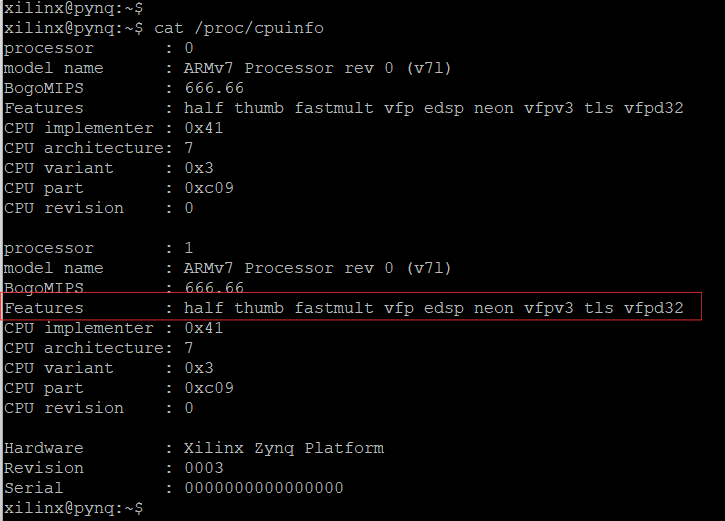
\includegraphics[width=0.75\textwidth]{zc702_cpuinfo.png}
\caption{Confirming directly on the board that this processor is missing the math instruction the published software assumed it would have.}
\label{fig:cpuinfo}
\end{figure}

The fix was to rebuild that software from scratch on the board itself, targeting the processor's real capabilities. This meant building a basic tool from scratch first too, since the board's software was too old to have one ready-made. Building it natively, rather than elsewhere and copying it across, let the process detect exactly what the chip supports rather than guessing. This solved the crash, confirmed by comparing predictions directly against the reference version (Section~\ref{sec:qr-runtime-correctness}).

\section{FPGA alert-controller design and verification}
\label{sec:fpga-alert-design}

A full hardware version of the classifier was considered early on, in line with a fallback plan, but judged unlikely to reach a working state in the time available \citep{lu2025hardware,parra2023methodology}. Instead, the hardware work focuses on the stage right after the classifier: turning a raw prediction into an alert. This was built as a small circuit that only raises an alert after eight confident "distracted" readings in a row and clears it after eight confident "safe" readings in a row, matching the same cut-off already proven in the software version. Reusing an already-working idea in hardware, rather than a separate rule, keeps the design grounded in something already shown to work.

This was checked two ways. A standalone test ran the logic against ten made-up edge cases and 28 real predictions from the trained model, including two real mistakes it made, were replayed through a simulated version of the full link between camera, processor and alert circuit, to check the design handles real, imperfect data. The circuit was then built for a low-cost board, chosen deliberately as an affordable target, using Vivado 2017.4 in batch mode. The full design is in Appendix~\ref{app:code}, Listing~\ref{lst:verilog-controller}.

\section{Alert delivery, tools and test strategy}

To turn a detection into something a driver or fleet manager would see, the board runs a continuous capture-classify-alert loop, using the same logic as the hardware version above. Every alert, with the photo that triggered it, is sent to a small server, which notifies a phone app. A buzzer wired to the board gives a second, independent alert at the same moment, so a driver is warned even without a phone nearby. This needed a small custom hardware addition, built, tested and loaded onto the board, exposing a control pin with no way of being switched on before \citep{xilinx2019ug850} - the one part of this project's hardware work tested on real equipment rather than estimated (Section~\ref{sec:qr-fpga}). Full detail and the three layers the alert path was checked in, are in Appendix~\ref{app:buzzer} and Appendix~\ref{app:alertpath}.

The AI side used Python and standard machine-learning tools; the hardware side used the manufacturer's own design software and the board's Linux environment. Testing happened at every stage, not just the end. Each dataset was checked immediately after being added, for missing labels, lost images, or a driver appearing in more than one split, exactly what caught a real bug early on. Every accuracy figure comes from data the model never saw during training. The conversion was checked both structurally and by confirming matching output and the same standard was applied on the board, checking predictions actually matched rather than assuming a crash disappearing meant everything was correct.

\section{Ethical, legal, professional and social issues}

Formal ethics approval was not required because the experiments used existing public datasets \citep{statefarm2016dataset,yang2024samdd,saad2020dataset}, together with limited test footage recorded by the researcher. No participants were recruited and no third-party personal data were collected. The datasets were stored locally rather than redistributed, in accordance with their licences; one dataset is restricted to non-commercial use.

The available datasets do not provide sufficient demographic information to assess performance fairly across age, ethnicity or body type. No claim of demographic fairness is therefore made. Driver monitoring also creates a privacy concern because a camera continuously observes the driver. Local processing reduces this risk because ordinary footage remains on the device, although the current prototype sends the image associated with an alert. A practical product should allow that feature to be disabled and should apply clear retention and access controls.

Both missed distractions and false alerts have safety consequences. Repeated false alerts may cause users to ignore or disable the system, which is why the decision logic requires several confident predictions before raising an alert. In line with the BCS Code of Conduct \citep{bcs2026conduct}, the system is presented as a research prototype rather than a finished safety product. Access to borrowed hardware also constrained the work, since experiments that risked damaging the board could not reasonably be attempted.







%!TEX root = main.tex

\chapter{Quality and Results}
\label{ch:results}

Every result in this chapter comes from the fixed held-out subjects listed in Table~\ref{tab:split-integrity}. Full per-class precision, recall and F1 tables for all six trained models are in Appendix~\ref{app:classreports}.

\section{Single-view baseline: model comparison (RQ1)}
\label{sec:qr-baseline}

Table~\ref{tab:model-comparison} shows the three architectures trained on State Farm under the subject-wise split. MobileNetV2 got the highest test accuracy (84.67\%) and macro F1 (84.01\%), ahead of EfficientNet-B0 (82.47\% / 81.58\%) and the custom CNN (75.60\% / 75.27\%). EfficientNet-B0's validation-to-test gap (72.23\% against 82.47\%) is worth noting, since by chance this validation split was harder than the test split for that model, and a single number should not be over-read under a protocol with only four drivers per partition, one reason Section~\ref{sec:eval-limitations} treats the lack of multi-seed data as a real limitation.

\begin{table}[htbp]
\centering
\caption{Single-view model comparison on the State Farm subject-wise test set (3{,}086 images, 4 held-out drivers).}
\label{tab:model-comparison}
\small
\begin{tabular}{lccccc}
\toprule
\textbf{Model} & \textbf{Val. acc.} & \textbf{Test acc.} & \textbf{Macro F1} & \textbf{Weighted F1} & \textbf{Train time (min)} \\
\midrule
Baseline CNN & 60.89\% & 75.60\% & 75.27\% & 76.57\% & 11.87 \\
MobileNetV2 & 82.12\% & \textbf{84.67\%} & \textbf{84.01\%} & \textbf{84.94\%} & 32.03 \\
EfficientNet-B0 & 72.23\% & 82.47\% & 81.58\% & 82.79\% & 37.57 \\
\bottomrule
\end{tabular}
\end{table}

\begin{figure}[htbp]
	\centering
	\begin{subfigure}{0.49\textwidth}
		\centering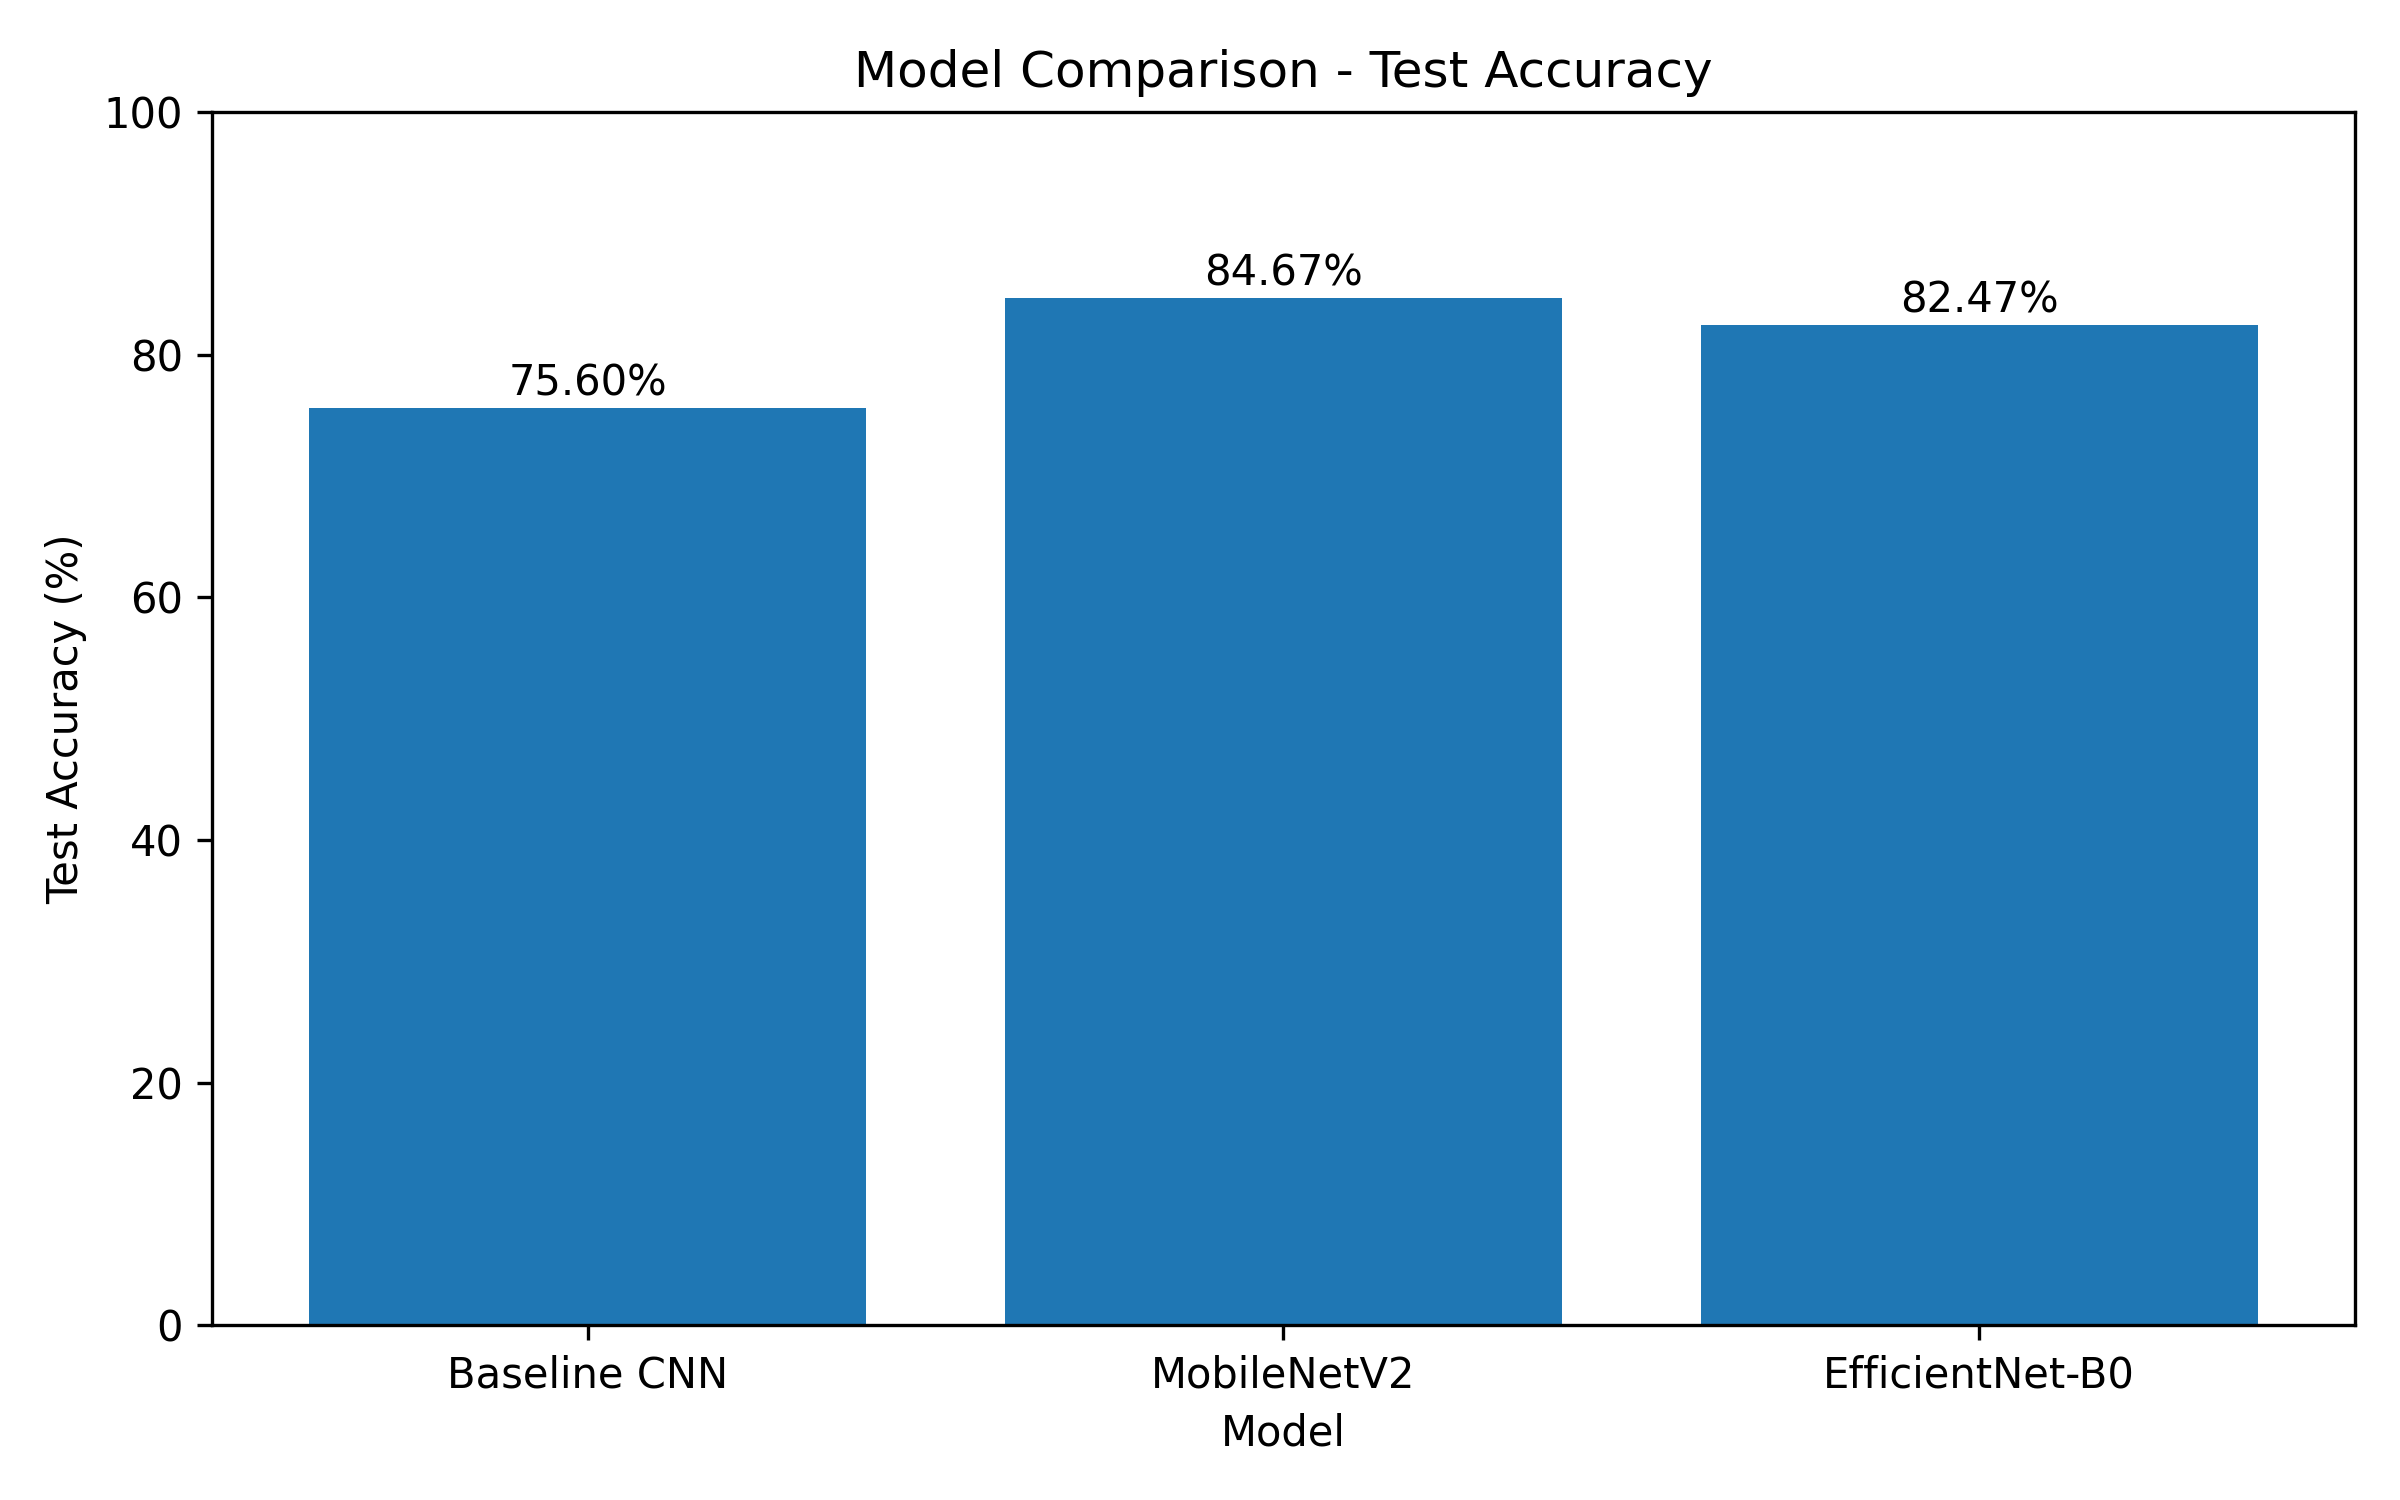
\includegraphics[width=\linewidth]{model_comparison_test_accuracy.png}
		\caption{Test accuracy}
	\end{subfigure}
	\hfill
	\begin{subfigure}{0.49\textwidth}
		\centering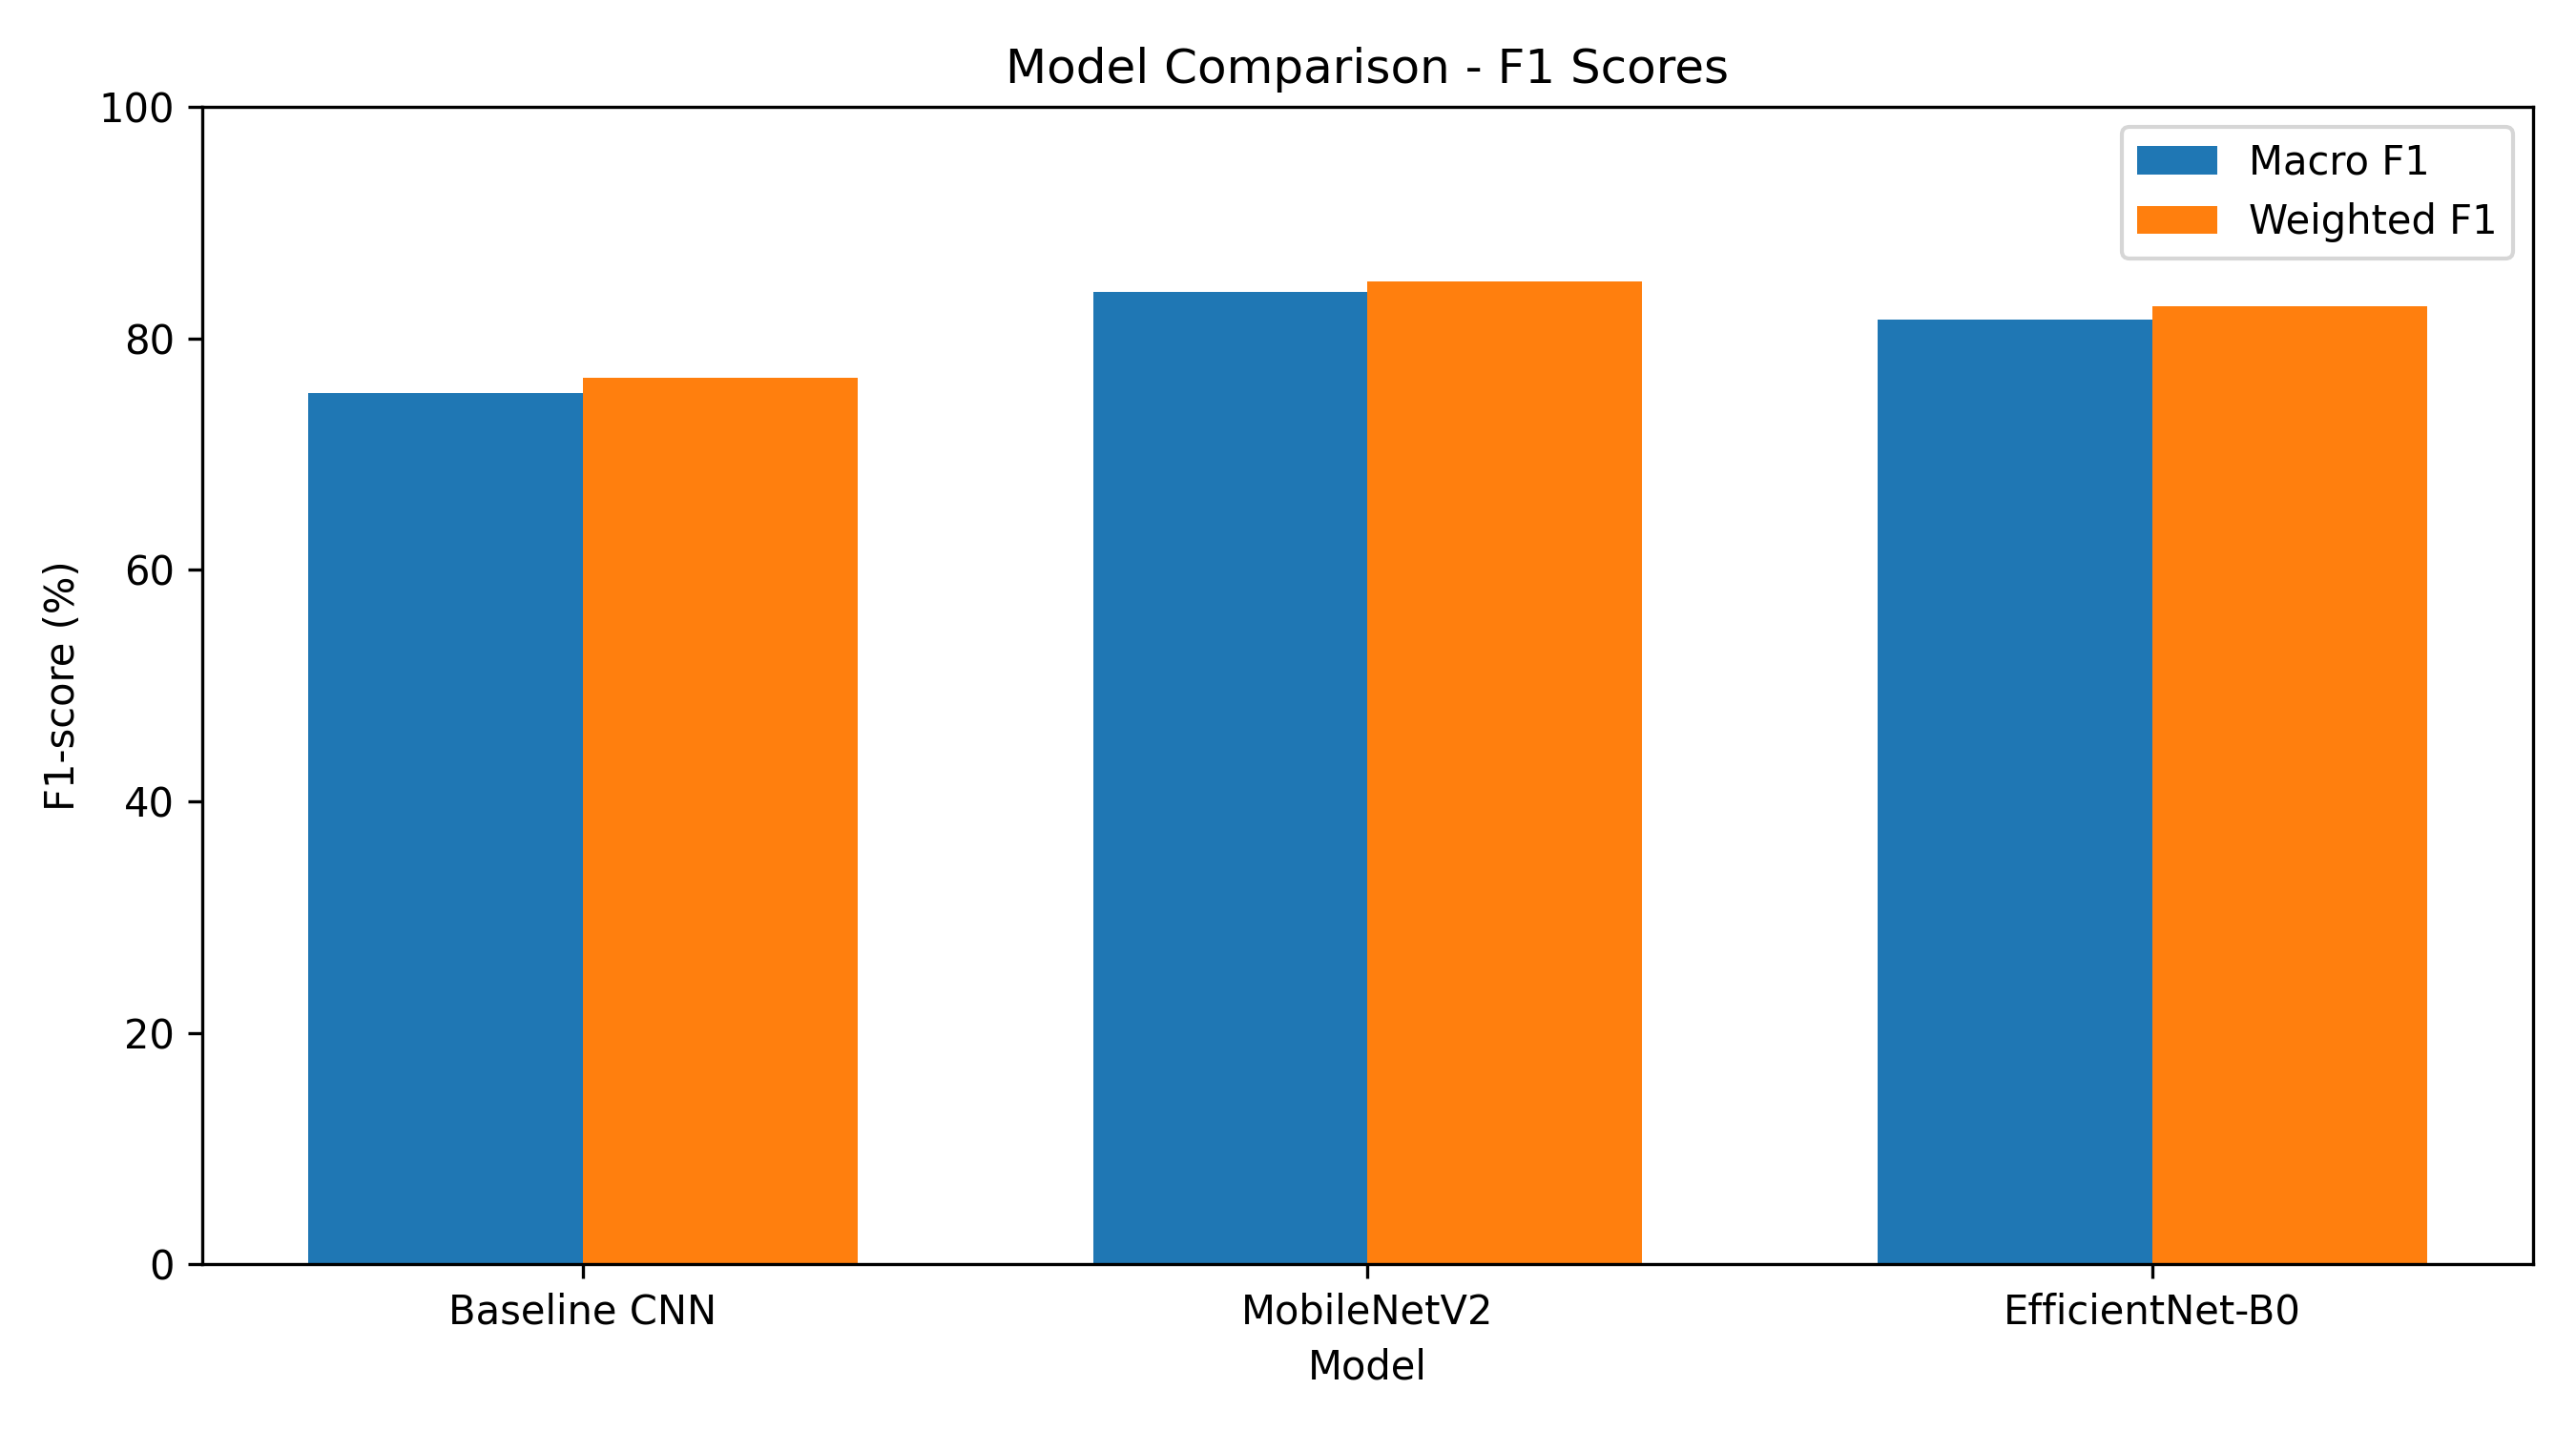
\includegraphics[width=\linewidth]{model_comparison_f1_scores.png}
		\caption{Macro and weighted F1}
	\end{subfigure}
	\caption{Single-view model comparison across accuracy and F1 metrics.}
	\label{fig:model-comparison}
\end{figure}

Deployment-oriented measurements (Table~\ref{tab:deployment}, Figure~\ref{fig:acc-vs-fps}) were taken on the development laptop, not embedded hardware, and that comparison appears separately in Section~\ref{sec:qr-consolidated}. MobileNetV2 was not the fastest model here (16.64 FPS against the custom CNN's 17.61 FPS), but its nine-point accuracy advantage is why it was carried forward, a clear trade-off between accuracy, throughput and size, not a claim that it wins on every measure.

\begin{table}[htbp]
\centering
\caption{Deployment-oriented measurements on the development laptop (GPU-accelerated). These are laptop figures and are not comparable with the on-device figures in Table~\ref{tab:consolidated}.}
\label{tab:deployment}
\small
\begin{tabular}{lccc}
\toprule
\textbf{Model} & \textbf{Size (MB)} & \textbf{Inference (ms)} & \textbf{Throughput (FPS)} \\
\midrule
Baseline CNN & 4.96 & 56.79 & 17.61 \\
MobileNetV2 & 20.78 & 60.08 & 16.64 \\
EfficientNet-B0 & 15.75 & 64.51 & 15.50 \\
\bottomrule
\end{tabular}
\end{table}

\RequiredFigure[0.80\textwidth]{accuracy_vs_fps_all_models.png}{Accuracy against laptop throughput for the three baseline models, showing the trade-off underlying the MobileNetV2 selection.}{fig:acc-vs-fps}

A small qualitative test on out-of-domain photographs taken by the researcher showed domain shift directly. All three models classified a dataset-style image correctly, but across three independently captured photographs only EfficientNet-B0 got two of three actions right, MobileNetV2 got one, and the custom CNN got none. With only three images this is no substitute for the quantitative evaluation that follows, but it was the first sign that strong within-distribution accuracy does not prove robustness to a changed context, and it motivated both robustness stages.

\section{Cross-view generalisation (RQ2)}
\label{sec:qr-crossview}

MobileNetV2 was retrained on the unified State Farm and SAM-DD table (80{,}211 training images spanning \texttt{side} and \texttt{front}) with the backbone frozen. Mixed-view accuracy reached only 75.94\%, and it was clearly uneven, 78.79\% on \texttt{front} against 73.93\% on \texttt{side}. A model not trained on purpose to be view-robust is not automatically view-robust, even when both views are present in its training data, and the two are not handled equally well by default.

Unfreezing the last 30 layers and fine-tuning at $1\times10^{-5}$ improved every measure (Table~\ref{tab:crossview}). Early stopping restored the epoch-5 weights, where validation accuracy peaked at 91.24\%, and training accuracy had already gone past 98\% by epoch 3, so later epochs were overfitting (Figure~\ref{fig:crossview-curves}).

\begin{table}[htbp]
\centering
\caption{Cross-view MobileNetV2 accuracy, frozen-backbone against fine-tuned, on the 17{,}992-image held-out mixed-view test set.}
\label{tab:crossview}
\small
\begin{tabular}{lccc}
\toprule
\textbf{Test partition} & \textbf{Frozen-backbone} & \textbf{Fine-tuned} & \textbf{Change} \\
\midrule
Mixed-view (17{,}992 images) & 75.94\% & \textbf{91.76\%} & $+15.8$ pt \\
\texttt{side} view (10{,}539 images) & 73.93\% & \textbf{91.05\%} & $+17.1$ pt \\
\texttt{front} view (7{,}453 images) & 78.79\% & \textbf{92.77\%} & $+14.0$ pt \\
\bottomrule
\end{tabular}
\end{table}

\RequiredFigure[0.92\textwidth]{mobilenetv2_crossview_training_curves.png}{Cross-view MobileNetV2 training curves for both phases, with the restored best epoch marked.}{fig:crossview-curves}

\RequiredFigure[0.92\textwidth]{mobilenetv2_crossview_confusion_matrices.png}{Cross-view confusion matrices before and after fine-tuning, mixed-view held-out test set.}{fig:crossview-confusion}

All ten classes improved, but unevenly, and this unevenness is actually the more useful result (Section~\ref{sec:qr-class-errors}). Figure~\ref{fig:crossview-qualitative} shows predictions on real held-out images from both views.

\RequiredFigure[0.82\textwidth]{mobilenetv2_crossview_qualitative_samples.png}{Qualitative predictions from the fine-tuned cross-view model on held-out test images spanning both camera views.}{fig:crossview-qualitative}

\section{Lighting-domain robustness (RQ3)}
\label{sec:qr-lowlight}

This stage asks what happens to a day-trained model on real night-time footage captured under active infrared light, not a synthetically darkened daylight image. The results here are the most severe in the whole project.

\subsection{The day-only baseline collapses}

The best single-view State Farm MobileNetV2 checkpoint, the same model that got 84.67\% on its own daytime test set, was tested directly on the 1{,}500 held-out real night images with zero retraining. It scored 19.53\%.

That number actually understates how bad the failure is. This is not degradation spread across ten classes, it is a collapse. The model puts almost every night image into just two classes, reaching 99.3\% recall on \texttt{texting\_left} and 96.0\% on \texttt{reaching\_behind}, while recording 0.0\% recall on the other eight (Appendix~\ref{app:classreports}). It has not just become confused, it has lost the ability to tell classes apart completely, and this is arguably worse than random guessing, since a downstream alert stage would receive a stream of confident, consistent, wrong classifications rather than obvious noise.

\subsection{Training on real night data recovers most of the gap}

A fresh MobileNetV2 was then trained on the merged table, 20{,}399 training images, State Farm daytime plus only the real night subset, for the reason explained in Section~\ref{sec:method-lowlight-data}. It used the same protocol as the cross-view stage, so the two robustness results can be compared directly.

\begin{table}[htbp]
\centering
\caption{Lighting-domain robustness. The baseline column is the day-trained model applied to night images with no retraining. All test figures come from held-out drivers.}
\label{tab:lowlight}
\small
\begin{tabular}{lccc}
\toprule
\textbf{Test partition} & \textbf{Day-only baseline} & \textbf{Frozen-backbone} & \textbf{Fine-tuned} \\
\midrule
Mixed day+night (4{,}586 images) & --- & 62.30\% & \textbf{77.91\%} \\
\texttt{day} (3{,}086 images) & 84.67\%\textsuperscript{$\dagger$} & 64.55\% & \textbf{81.21\%} \\
\texttt{night} (1{,}500 images) & 19.53\% & 57.67\% & \textbf{71.13\%} \\
\bottomrule
\multicolumn{4}{l}{\footnotesize \textsuperscript{$\dagger$}On its own single-domain State Farm test set, shown for reference.}
\end{tabular}
\end{table}

First, training a new classification head on real day and night data, with the backbone still at ImageNet weights, lifts night accuracy from 19.53\% to 57.67\%, meaning most of the collapse was a classifier-layer problem, not proof ImageNet features are useless on infrared-illuminated images. Second, fine-tuning recovers most of what is left, and night accuracy reaches 71.13\%, a gain of 51.6 points over the untreated baseline, done with real captured footage, not a synthetic approximation.

Third, this is a trade-off, not a free win. Even after fine-tuning, day accuracy reaches only 81.21\%, 3.5 points below the 84.67\% the original single-domain model got on the same test set, since training one shared classifier across both lighting domains costs some single-domain performance to buy cross-domain robustness. This negative transfer is small but real, worth stating plainly rather than describing only the night improvement.

\RequiredFigure[0.92\textwidth]{mobilenetv2_lowlight_training_curves.png}{Low-light MobileNetV2 training curves for both phases. Both ran their full ten epochs, and the best epoch of the fine-tuning phase was the last.}{fig:lowlight-curves}

\RequiredFigure[0.92\textwidth]{mobilenetv2_lowlight_confusion_matrices.png}{Low-light confusion matrices for the day-only baseline, frozen-backbone and fine-tuned models. The baseline's collapse into two predicted classes is visible as two dominant columns.}{fig:lowlight-confusion}

\RequiredFigure[0.80\textwidth]{mobilenetv2_lowlight_qualitative_samples.png}{Qualitative predictions from the fine-tuned low-light model on held-out real night-time images.}{fig:lowlight-qualitative}

\section{Quantisation: accuracy, size and latency (RQ4)}
\label{sec:qr-quantisation}

Quantisation is what makes embedded deployment possible at all. Its cost is reported here across all four measures the interim feedback asked for, accuracy, size, latency and throughput, before and after conversion.

\subsection{Model size}

The fine-tuned cross-view Keras model is 21{,}791{,}872 bytes (20.78~MB), and the INT8 TensorFlow Lite conversion is 2{,}723{,}448 bytes (2.60~MB), a compression ratio of \textbf{8.00$\times$}. This is what INT8 quantisation of a mostly float32 model should give, confirming the conversion worked as intended rather than quietly keeping the float weights.

\subsection{Accuracy}

Two before-and-after comparisons were measured on different samples, and both are reported here because the difference between them is informative on its own (Table~\ref{tab:quantisation-accuracy}).

\begin{table}[htbp]
\centering
\caption{Quantisation accuracy cost, measured on different held-out samples. The two loss figures differ because INT8 quantisation error is data-dependent, not because either measurement is unreliable.}
\label{tab:quantisation-accuracy}
\small
\begin{tabular}{llccc}
\toprule
\textbf{Model} & \textbf{Evaluation sample} & \textbf{Keras float32} & \textbf{TFLite INT8} & \textbf{Cost} \\
\midrule
Cross-view, frozen & 500 mixed-view images & 76.80\% & 76.00\% & $-0.8$ pt \\
Cross-view, frozen & 300 random \texttt{side} images & 59.30\% & 54.70\% & $-4.6$ pt \\
Cross-view, fine-tuned & 300 random \texttt{side} images & 80.00\% & 77.30\% & $-2.7$ pt \\
\bottomrule
\end{tabular}
\end{table}

The first was made at conversion time on a 500-image mixed front-and-side sample, and showed only a 0.8-point cost. The second used a 300-image random draw from the \texttt{side} test split, not deliberately balanced, and showed a 4.6-point cost on the same model. These two do not disagree, since INT8 error depends on the data it is measured over, and the 300-image draw is simply harder. The unquantised model itself only scores 59.3\% on it, well below the 73.93\% \texttt{side} average, which is why it was investigated rather than treated as a deployment fault.

The third row matters most, since the fine-tuned model is what was actually deployed. Quantisation costs \textbf{2.7 points} on the same 300 images that cost the frozen model 4.6, and the smaller cost on the better-trained model fits with the idea that larger prediction margins are more tolerant of quantisation noise. Both figures sit within the few-point range \citet{abushahla2025quantization} report as typical.

\subsection{The consolidated software-to-hardware comparison}
\label{sec:qr-consolidated}

Table~\ref{tab:consolidated} brings the whole pipeline into one place, the laptop float32 reference, the laptop-converted INT8 model, and that same model running on real ZC702 hardware, with the separate FPGA-fabric figures next to them. Keeping laptop and hardware performance clearly apart is the whole point of this table.

\begin{table}[htbp]
\centering
\caption{Consolidated software, deployment and hardware comparison for the fine-tuned cross-view MobileNetV2 and the FPGA alert controller. Laptop and on-device figures are reported separately and are not interchangeable.}
\label{tab:consolidated}
\footnotesize
\begin{tabular}{llccc}
\toprule
\textbf{Stage} & \textbf{Platform} & \textbf{Model size} & \textbf{Accuracy\textsuperscript{a}} & \textbf{Latency / throughput} \\
\midrule
Reference (float32) & Laptop (RTX 3060) & 20.78 MB & 80.0\% & 60.08 ms / 16.64 FPS\textsuperscript{b} \\
Quantised (INT8) & Laptop (converted) & 2.60 MB & 77.3\%\textsuperscript{c} & not separately timed \\
Deployed (INT8) & ZC702 (Cortex-A9) & 2.60 MB & \textbf{77.3\%} & \textbf{9{,}150 ms / 0.11 FPS} \\
\midrule
\multicolumn{5}{l}{FPGA fabric, alert-decision stage only, not the CNN (post-synthesis, \texttt{xc7a35tcpg236-1}):} \\
\multicolumn{5}{l}{18 LUTs (0.09\%) $\cdot$ 13 FFs (0.03\%) $\cdot$ 0 BRAM $\cdot$ 0 DSP $\cdot$ $+7.276$ ns slack at 100 MHz} \\
\bottomrule
\multicolumn{5}{p{0.95\textwidth}}{\footnotesize \textsuperscript{a}Same 300-image held-out \texttt{side} sample throughout, so the rows are directly comparable. \textsuperscript{b}Laptop latency was measured for this architecture during the baseline evaluation. The fine-tuned model is the same architecture and input size, so the figure carries over, but it was not separately re-timed. \textsuperscript{c}The laptop-converted and on-device INT8 models agreed on 100 of 100 predictions, so they share an accuracy figure by measurement, not assumption.}
\end{tabular}
\end{table}

Quantisation buys an 8$\times$ size reduction for a cost of 2.7 accuracy points. Moving from laptop to the embedded target costs almost nothing in accuracy, since the INT8 model behaves the same on both, but it costs roughly \textbf{150$\times$ in speed}. The fabric alert-decision stage is meanwhile almost free, so the pipeline's whole cost sits in the CNN, exactly the reason a dedicated CNN accelerator would make sense as the next engineering step (Section~\ref{sec:eval-future}).

\section{On-device deployment on the ZC702 (RQ4)}
\label{sec:qr-ondevice}

\subsection{Establishing runtime correctness first}
\label{sec:qr-runtime-correctness}

Before any on-device accuracy figure could be trusted, the from-source runtime (Section~\ref{sec:arm32-issue}) had to be shown numerically correct, not just crash-free. An early board-versus-laptop comparison showed only 71\% agreement, which looked like a broken build but was not, since the cause was the test script, which resized images with \texttt{PIL.Image.resize()} while training had used \texttt{tf.image.resize()}. The deployment script itself was unaffected, since it already used \texttt{cv2.resize}, matching \texttt{tf.image.resize} 95\% of the time. Once preprocessing was matched, board-versus-reference agreement was \textbf{100 out of 100}, every prediction identical, which shows the rebuilt ARM32 runtime is numerically faithful to the official implementation, a stronger claim than just saying it does not crash.

\subsection{Accuracy on real hardware}

A 300-image random sample was then evaluated four ways, Keras float32 and on-device TFLite INT8, for both the frozen and fine-tuned checkpoints (Figure~\ref{fig:ondevice-accuracy}). Fine-tuning improved on-device accuracy from 54.7\% to \textbf{77.3\%}, a gain of 22.6 points measured on real hardware, not just assumed from lab results, which shows the lab improvement survives quantisation and deployment fully intact, not something that could be assumed in advance.

\RequiredFigure[0.74\textwidth]{zc702_ondevice_accuracy_comparison.png}{On-device (ZC702, TFLite INT8) against reference (Keras float32) accuracy on the same 300-image held-out sample, before and after fine-tuning.}{fig:ondevice-accuracy}

On-device inference took about 9.15 seconds per image, with XNNPACK acceleration turned off on purpose, the known-safe setting this ARM32 target's crash fix was verified under, and the clearest limitation of this deployment. Section~\ref{sec:eval-challenges} explains why re-enabling XNNPACK was looked into but not attempted.

\section{FPGA alert-controller verification and synthesis (RQ5)}
\label{sec:qr-fpga}

Both testbenches passed in full. The standalone hysteresis testbench passed all ten checks, and the end-to-end testbench replayed 28 real classification outputs over a simulated UART link, including two real model misclassifications, both correctly absorbed without setting off a false alert, exactly the failure mode the design exists to prevent, tested against real wrong model output, not synthetic noise. Out-of-context synthesis for the Artix-7 target (Table~\ref{tab:fpga}, Figure~\ref{fig:fpga-util}) shows the controller uses a tiny fraction of the device and meets its 100~MHz timing constraint with 7.276~ns of slack to spare.

\begin{table}[htbp]
\centering
\caption{Post-synthesis results for the alert controller, \texttt{xc7a35tcpg236-1}, out-of-context. Raw report excerpts are in Appendix~\ref{app:fpga}.}
\label{tab:fpga}
\small
\begin{tabular}{lr}
\toprule
\textbf{Metric} & \textbf{Value} \\
\midrule
Slice LUTs & 18 (0.09\% of 20{,}800) \\
Slice registers (flip-flops) & 13 (0.03\% of 41{,}600) \\
Block RAM & 0 \\
DSP slices & 0 \\
Worst negative slack at 100 MHz & $+7.276$ ns \\
Worst hold slack & $+0.272$ ns \\
Failing timing endpoints & 0 of 17 \\
Implied theoretical maximum frequency & $\sim$367 MHz \\
Estimated total on-chip power & 0.069 W (0.068 W static) \\
\bottomrule
\end{tabular}
\end{table}

\RequiredFigure[0.78\textwidth]{fpga_synthesis_utilization.png}{Post-synthesis resource utilisation for the alert controller on \texttt{xc7a35tcpg236-1}.}{fig:fpga-util}

First, these are post-synthesis estimates, not measurements from a design actually placed and routed on physical silicon, since this project never had access to a real Artix-7 board, and the target was chosen as a typical low-cost device. Vivado's own report says final LUT counts after physical optimisation are usually lower, so if anything this figure is conservative, but it is still an estimate. Second, the power figure is a vector-less estimate at the tool's own medium confidence level. Third, and this matters most, these numbers describe the decision stage only, not the CNN, since the classifier runs in software on the ARM core and is not part of this synthesised design, so nothing in Table~\ref{tab:fpga} should be read as the resource cost of running MobileNetV2 in fabric.

What the FPGA work does prove is narrower, but real. The logic that turns a noisy prediction stream into a stable alert is a lightweight, low-power part that fits on the cheapest FPGA devices, verified against real model output including real errors, and reproducible from the scripts submitted with this report.

\section{Class-level error analysis across all three stages}
\label{sec:qr-class-errors}

Reporting only the headline accuracy would hide the more useful structure in these results. Table~\ref{tab:class-errors} tracks the most diagnostic classes.

\begin{table}[htbp]
\centering
\caption{Selected per-class results across stages (P = precision, R = recall). Full tables in Appendix~\ref{app:classreports}.}
\label{tab:class-errors}
\small
\begin{tabular}{lcccccc}
\toprule
& \multicolumn{2}{c}{\textbf{Cross-view frozen}} & \multicolumn{2}{c}{\textbf{Cross-view fine-tuned}} & \multicolumn{2}{c}{\textbf{Low-light fine-tuned}} \\
\cmidrule(lr){2-3}\cmidrule(lr){4-5}\cmidrule(lr){6-7}
\textbf{Class} & \textbf{P} & \textbf{R} & \textbf{P} & \textbf{R} & \textbf{P} & \textbf{R} \\
\midrule
\texttt{talking\_to\_passenger} & 0.61 & 0.14 & 0.60 & 0.52 & 0.72 & 0.82 \\
\texttt{texting\_left} & 0.42 & 0.77 & 0.97 & 0.82 & 0.97 & 0.65 \\
\texttt{texting\_right} & 0.69 & 0.50 & 0.92 & 0.77 & 0.99 & 0.46 \\
\texttt{hair\_or\_makeup} & 0.70 & 0.54 & 0.87 & 0.88 & 0.60 & 0.66 \\
\texttt{drinking} & 0.75 & 0.61 & 0.84 & 0.83 & 0.64 & 0.89 \\
\texttt{safe\_driving} & 0.89 & 0.88 & 0.94 & 0.98 & 0.55 & 0.85 \\
\bottomrule
\end{tabular}
\end{table}

\texttt{hair\_or\_makeup} is the hardest class in the project, not tied to one robustness condition, weakest in the single-view baseline (F1 0.71), weakest again in the low-light frozen model (F1 0.42), and only 0.87 in the cross-view fine-tuned model. Raising a hand to the face looks visually close to several other classes, phone-to-ear in particular, and the object being held is small, often hidden, and the first thing lost when image quality drops.

\texttt{talking\_to\_passenger} improves a lot with fine-tuning but starts close to useless, recall rising from 13.6\% to 51.9\% in the cross-view model. It is also the smallest class in that test set, 258 examples against \texttt{safe\_driving}'s 9{,}006, making its recall the least stable figure in the project. Its stronger lighting-stage result (0.82 recall) is on a more balanced test set and should not be read as this class suddenly becoming easy.

\texttt{texting\_left} in the cross-view frozen model gives the clearest signal here, precision 0.42 against recall 0.77, where high recall with poor precision means the model was using this class as a catch-all for other classes' predictions. Fine-tuning moved precision to 0.97 while recall stayed about the same, so the improvement came from better class boundaries, not a flat shift across the board, which is what makes the $+15.8$ point headline mean something rather than just being large.

\texttt{texting\_right} in the low-light fine-tuned model shows the opposite imbalance, more likely a labelling problem than a modelling one, precision 0.99 against recall 0.46, reliable whenever it predicts the class but missing more than half the true instances, the pattern expected if a chunk of examples were labelled inconsistently, matching the hand-side ambiguity Section~\ref{sec:method-lowlight-data} documents for these four classes. This is the most likely explanation, not a proven one, and telling a real weakness apart from label noise would need a re-checked subset, which was not available here.

\section{Summary against the research questions}
\label{sec:qr-rq-summary}

\begin{description}[leftmargin=1.5em,style=nextline,itemsep=0.15em]
	\item[RQ1 --- Model comparison.] MobileNetV2 outperformed both alternatives under subject-wise evaluation (84.67\% accuracy, 84.01\% macro F1) while remaining the most deployable on size and throughput together (\S\ref{sec:qr-baseline}).
	\item[RQ2 --- Cross-view robustness.] A simply pooled multi-view model shows a real, uneven gap (75.94\% mixed, \texttt{side} 4.9 points behind \texttt{front}). Fine-tuning closes most of it, up to 91.76\%, and the class-level evidence shows the gain came from better class boundaries, not a flat shift across the board (\S\ref{sec:qr-crossview}, \S\ref{sec:qr-class-errors}).
	\item[RQ3 --- Lighting robustness.] A day-trained model collapses to 19.53\% on real infrared-illuminated night footage, with zero recall on eight of ten classes. Real night training recovers this to 71.13\%, at a cost of 3.5 points of daytime accuracy (\S\ref{sec:qr-lowlight}).
	\item[RQ4 --- Quantisation and deployment cost.] INT8 conversion reduces the model 8.00$\times$ for 2.7 accuracy points, and it is numerically identical on board and laptop. The embedded target costs roughly 150$\times$ in speed (\S\ref{sec:qr-quantisation}, \S\ref{sec:qr-ondevice}).
	\item[RQ5 --- What is credibly implementable in fabric.] The decision stage, not the classifier. It was verified against real model predictions, including real misclassifications, and synthesised at 18 LUTs and 13 flip-flops with 7.276~ns of positive slack. These are post-synthesis estimates, not measurements on physical silicon (\S\ref{sec:qr-fpga}).
\end{description}

%!TEX root = main.tex

\chapter{Evaluation and Conclusion}
\label{ch:evaluation}

\section{Final evaluation against objectives}
\label{sec:eval-objectives}

Both objectives set out in Chapter~\ref{ch:introduction} were met, though not in the shape originally planned.

The first objective, preparing and using real multi-view and real low-light data, was met in full. The multi-view part went as planned. The lighting part did not, since it was planned as synthetic infrared-like augmentation and was replaced on purpose with training on real captured night footage once that data became available. This directly answers the interim supervisor feedback, which warned that synthetic low-light transforms should be described as an approximation of robustness, not a substitute for real infrared data. Rather than relabelling the experiment to satisfy this, it was replaced with one that does not need the caveat at all.

The second objective, a prototype on real, low-cost embedded hardware with an alert output reacting to sustained rather than momentary predictions plus a measured account of what getting there costs, was also met, though the hardware path changed along the way. The original plan treated a full FPGA-fabric CNN accelerator as the main goal, with a software fallback as backup. What was actually built runs the CNN on the ZC702's ARM core and only uses the fabric for the decision stage, a considered decision about scope, not a fallback settled for reluctantly. A dedicated accelerator is a multi-week job even starting from an existing architecture \citep{lu2025hardware}, and the IPR had already flagged this trade-off before it came up.

The quantification work answers that feedback most directly, since it asked that quantisation be checked through accuracy, model size, latency and throughput, before and after conversion, with laptop FPS clearly kept apart from hardware performance. Section~\ref{sec:qr-quantisation} reports all four measures with real numbers, and Table~\ref{tab:consolidated} gives the single combined comparison also asked for, with laptop and on-device rows kept separate rather than blended into one throughput claim.

\section{Project management}

The timeline set at the start (May to September 2026, single-view work through July, hardware work in August and September) fell short in one way, it did not expect robustness to become two full stages rather than one small check. Both were added after the qualitative domain-shift test in Section~\ref{sec:qr-baseline} made the problem real instead of theoretical. Looking back this was the right call, since the two robustness results are arguably the more original part of this project, but it did compress the hardware phase, a direct cause of later decisions, running the CNN on the ARM core instead of building a custom accelerator, and leaving the XNNPACK question unresolved. The lesson here is that a robustness finding worth investigating properly needs its own budgeted time from the start, not squeezed into an existing timeline once found. A second lesson is about ordering, since the lighting stage was the last big piece of work finished, leaving no room for it to go wrong. It did not, but that was not a margin the plan had earned.

\section{Insights gained}
\label{sec:eval-insights}

The most important technical insight was that a crash on unfamiliar embedded hardware is not necessarily proof the approach cannot work, it can just as easily be evidence of a specific, diagnosable, fixable mismatch between a generic published tool and the exact hardware in front of you. Giving up on on-device inference after the first \texttt{Illegal instruction} crash was a reasonable call given the information available at the time. Reopening that decision, working out the VFPv3-against-VFPv4 mismatch, and rebuilding the runtime from source on the board best shows the difference between treating an obstacle as a dead end and treating it as a problem with a findable cause.

The second insight is that robustness does not just show up on its own from seeing varied data. The frozen-backbone cross-view model saw both camera views during training and still showed a large, uneven gap, and the frozen-backbone low-light model saw both lighting conditions and still trailed by seven points on night data. Both problems needed the backbone itself to be adapted, and in both cases the real size of the problem would have stayed invisible if only the after-fix number had been measured. Reporting the ``before'' figure on purpose is what carries most of the analytical value here.

A third insight is that what looks like a model or hardware problem is sometimes a data-pipeline problem in disguise. Both the preprocessing mismatch (Section~\ref{sec:qr-runtime-correctness}) and the night-driver split bug were exactly this kind of error, and both would have produced confident, believable, wrong numbers instead of an obvious failure.

\section{Reflection on challenges}
\label{sec:eval-challenges}

Two more challenges, beyond the ARM32 runtime issue, are worth reflecting on honestly here, rather than just reporting how they were resolved.

The first is the WiFi adapter that was meant to give the board its own connectivity, and it was never made to work. The first idea was a USB power-budget limit, since several peripherals shared one port through unpowered hubs chained together, so it was tested directly. The competing devices were switched off, removing 1~A of demand, and the driver was re-bound with the whole bus available to it. The failure was byte-for-byte identical, the same four register-access timeouts at the same four offsets, real evidence against the power-budget theory, which shifted the diagnosis to a real driver or chipset incompatibility instead. The honest outcome is a disproven guess and a still-unfixed problem, deprioritised since on-device inference needs no network at runtime, with the value in having tested the guess rather than just asserting it.

The second is inference speed. The fix for the original crash, compiling with \texttt{-march=native}, should in theory also let XNNPACK's runtime CPU dispatch avoid the same mismatch, since it uses the same detection library already working correctly for the compiled NEON kernels, but ``should in theory'' is not the same as ``checked and confirmed''. Some XNNPACK ARM32 source files fix FPU flags directly rather than relying on runtime dispatch, and checking this properly would have needed a multi-hour rebuild that carried real risk to a working installation the demo depended on. Risking a working deployment for a speed gain this close to a deadline was not a good trade, so this is a reasoned decision not to chase the lead, not an unexamined gap.

\section{Comparison to the literature}

Chapter~\ref{ch:litreview} pointed out that the cross-view literature mostly reports post-fix accuracy with no equivalent unfixed baseline. This project's frozen-against-fine-tuned comparison (75.94\% to 91.76\%) points the same way as \citet{bhalla2025crossview} and \citet{sengar2023poseviNet}, even though both use more advanced methods. What this project adds is the size of the untreated gap on a standard architecture, something those papers do not report, and something needed to judge how much of any published improvement actually comes from the method rather than just from having multi-view data at all.

On lighting, the 19.53\% collapse is more extreme than the gradual drop \citet{wang2023driver} report across different recording conditions, and gives a real measured reference point for the concern behind \citet{shen2023visible}'s image-translation work. The problem their synthetic approach exists to reduce is severe enough to justify the effort, and the fact that real night data recovers 51.6 points suggests real data is still the stronger fix where it can be obtained. On hardware, \citet{lu2025hardware}'s 13.05 FPS for a dedicated accelerator on the same XC7Z020 chip puts this project's 0.11 FPS in perspective. That gap of roughly two orders of magnitude is the direct cost of the decision not to build one. This project's hardware contribution was never going to be a faster result, it is a numerically verified one instead.

\section{Limitations}
\label{sec:eval-limitations}

Run-to-run variance was not measured, since every result comes from a single training run with a fixed random seed, so no confidence intervals can be given and small differences between conditions should not be read as reliably meaningful. The interim feedback specifically asked for uncertainty across runs, and this report cannot give that honestly, since the data simply does not exist, and generating it would have meant re-running each stage several times, roughly two hours per cross-view run alone, which the remaining time did not allow. Stating this gap directly is the right response, rather than making up an interval or quietly ignoring the request. It matters most for the smaller comparisons. The 3.5-point day-accuracy cost and the 2.2-point margin between MobileNetV2 and EfficientNet-B0 both sit in a range where seed variance could plausibly matter, while the 51.6-point night recovery and 15.8-point cross-view improvement are far too large to be explained that way.

Test partitions are small in terms of subjects. Four held-out State Farm drivers and two low-light night drivers are still a small group, however many images they produce, since images from the same driver are not independent samples of anything.

Label quality in two datasets is not perfect, and this is documented rather than hidden. SAM-DD's class mapping was rebuilt by visually checking images, with a confidence level recorded for each row, and four low-light classes still carry an unresolved hand-side problem. No demographic information exists in any dataset used here, so no fairness claim can be made either way, and SAM-DD is recorded on a simulator, not in a moving vehicle. The FPGA results are post-synthesis estimates covering the alert stage only. Two further datasets, AUC V2 and 100-Driver, were requested but not granted within the project timeline, so cross-view robustness here rests on two sources rather than four.

\section{Commercial context and future work}
\label{sec:eval-future}

The commercial case sketched out in Chapter~\ref{ch:introduction} still holds, with one big qualification. Component costs stay realistic for a retrofit or fleet product, the alert logic takes up under 0.1\% of a low-cost FPGA, the quantised model is 2.6~MB, and the classifier runs on ordinary ARM hardware. But 0.11 FPS is not a workable product figure. At roughly nine seconds per inference and eight ticks in a row needed before an alert fires, this setup would take over a minute to respond to sustained distraction, and that gap has to close before any commercial claim is believable. The non-technical risks are, if anything, bigger, since driver monitoring feels like surveillance to a lot of people rather than help, and false alerts create liability risk while training users to ignore the system.

Four directions follow from this. First, inference speed. Turning XNNPACK back on is a clear next step, and beyond that Table~\ref{tab:consolidated} makes the case for a dedicated CNN accelerator, since the pipeline's whole cost sits in the classifier. Second, stronger cross-domain methods, using the contrastive viewpoint-invariant approach from \citet{bhalla2025crossview} on the unified dataset built here, with the same idea applying to the lighting domain too. Third, broadening the data, since the AUC V2 and 100-Driver requests would add two more independent camera sources, and the 45{,}600 daytime infrared images left out of the lighting experiment would allow a three-way comparison, day-RGB, day-infrared and night-infrared, separating the lighting gap from the sensor-modality gap. Fourth, repeated-seed runs, to supply the variance data this report has to report as missing.

\section{Conclusion}

This project set out to test three connected claims. The first was that a classifier's accuracy under one camera view says nothing reliable about its accuracy under another. The second was that the same is true, even more so, for lighting. The third was that a complete, hardware-verified detection-and-alert pipeline is actually achievable on genuinely low-cost embedded hardware, not just estimated for it. All three held up.

A MobileNetV2 model trained under subject-wise evaluation reached 84.67\% on State Farm's side view, but showed a real, uneven cross-view gap when simply pooled across views. Fine-tuning on real paired multi-view data closed most of that gap, up to 91.76\%. The same model collapsed to 19.53\% on real captured infrared-illuminated night footage, a failure severe enough that the original plan to approximate it synthetically would have understated it, and training on real night data recovered this to 71.13\%, at a measured cost of 3.5 points of daytime accuracy. Quantisation compressed the deployed model eightfold for 2.7 accuracy points, proved numerically identical on board and laptop, and cost roughly 150$\times$ in speed. And a hardware decision stage was verified against real model predictions, including real misclassifications, synthesised at almost no cost on a low-cost FPGA target.

What connects these results is not any single number, it is a methodological position. Robustness is worth measuring before applying the fix, on real data rather than approximations of it, and on the actual hardware the claim is about rather than whatever hardware is convenient. Each of those choices gave a less flattering figure than the alternative would have, and each gave a more defensible one. For a system whose failures would happen inside a moving vehicle, that seems like the right way round.


% ============================================================
% REFERENCES
% ============================================================
\cleardoublepage
\phantomsection
\renewcommand{\bibname}{References}
\addcontentsline{toc}{chapter}{References}

\bibliographystyle{agsm}
\bibliography{paper}

% ============================================================
% APPENDICES
% ============================================================
\appendix
\renewcommand{\chaptername}{Appendix}
\addtocontents{toc}{\protect\vspace{0.5em}}

%!TEX root = main.tex

\chapter{Systematic Search and Screening Detail}
\label{app:prisma}

Supporting evidence for Section~\ref{sec:lit-prisma}. Literature search completed in June 2026. Table~\ref{tab:app-sources} shows the per-source distribution of the 90 records found before duplicates were removed. 

\begin{table}[H]
\centering
\caption{Search sources and initial records identified (before duplicate removal).}
\label{tab:app-sources}
\small
\begin{tabularx}{\textwidth}{lcY}
\toprule
\textbf{Source} & \textbf{Records} & \textbf{Main focus of results} \\
\midrule
IEEE Xplore & 32 & Driver distraction, CNNs, FPGA, low-light NoIR and IR/NIR studies \\
Google Scholar & 24 & Citation search, arXiv papers, dataset papers, review studies \\
SpringerLink & 8 & Driver monitoring, edge/cloud systems, deep learning \\
Elsevier / ScienceDirect-related & 8 & Intelligent systems, driver behaviour, accident-related monitoring \\
MDPI & 7 & Sensors, driver state monitoring, multimodal recognition \\
Dataset repositories, citation tracking & 6 & Mendeley low-light dataset, DMD, Zenodo dataset records \\
arXiv and preprint sources & 5 & DMD, edge AI, synthetic data, emerging methods \\
\midrule
\textbf{Total identified} & \textbf{90} & Records before duplicate removal \\
\bottomrule
\end{tabularx}
\end{table}

Exclusion criteria at the title and abstract screening stage include scope misalignment with camera-based driver monitoring, excessive generalization with no technical specifics, or technical incompleteness. Exclusion criteria at the full-text assessment stage include lack of dataset, methodology, evaluation result, or technical contribution. Inclusion criteria cover studies with RGB, low-light, NoIR, IR, NIR, depth, thermal, or multi-modal sensing, and studies providing dataset, camera setup, evaluation metric, or data split protocol.

\chapter{Dataset Splits and Composition}
\label{app:splits}

Supporting evidence for Section~\ref{sec:method-split-integrity} and Table~\ref{tab:split-integrity} is provided. Table~\ref{tab:app-sf-subjects} lists State Farm driver identifiers for each partition. These identifiers were set at the very beginning and used without changes in all baseline, cross-view, and lighting stages making sure that there was no driver migration between partitions throughout the whole project.

\begin{table}[H]
\centering
\caption{State Farm subject-wise split, by driver identifier.}
\label{tab:app-sf-subjects}
\small
\begin{tabularx}{\textwidth}{lccY}
\toprule
\textbf{Split} & \textbf{Images} & \textbf{Drivers} & \textbf{Driver identifiers} \\
\midrule
Train & 15{,}899 & 18 & p014, p015, p016, p021, p022, p024, p039, p042, p047, p049, p051, p052, p056, p061, p064, p066, p072, p081 \\
Validation & 3{,}439 & 4 & p026, p035, p041, p050 \\
Test & 3{,}086 & 4 & p002, p012, p045, p075 \\
\bottomrule
\end{tabularx}
\end{table}

\begin{table}[H]
\centering
\caption{Composition of the unified multi-view metadata table (170{,}316 rows).}
\label{tab:app-unified}
\small
\begin{tabular}{lllrrr}
\toprule
\textbf{Dataset} & \textbf{View} & \textbf{Lighting} & \textbf{Train} & \textbf{Val} & \textbf{Test} \\
\midrule
State Farm & side & day & 15{,}899 & 3{,}439 & 3{,}086 \\
SAM-DD & front & indoor artificial & 32{,}156 & 8{,}162 & 7{,}453 \\
SAM-DD & side & indoor artificial & 32{,}156 & 8{,}162 & 7{,}453 \\
Low-Light DD & side & night & 4{,}500 & 750 & 1{,}500 \\
Low-Light DD & side & day & 31{,}425 & 6{,}675 & 7{,}500 \\
\midrule
\multicolumn{3}{l}{Cross-view experiment (State Farm + SAM-DD)} & 80{,}211 & 19{,}763 & 17{,}992 \\
\multicolumn{3}{l}{Lighting experiment (State Farm + Low-Light night)} & 20{,}399 & 4{,}189 & 4{,}586 \\
\bottomrule
\end{tabular}
\end{table}

The rows of Low-Light DD daytime split are included into consolidated table but excluded from lighting experiment intentionally, in line with the reasoning provided in Section~\ref{sec:method-lowlight-data}. Figures~\ref{fig:app-sf-classes} and~\ref{fig:app-sf-subjects} show the distribution of State Farm classes and number of images per driver respectively.

\begin{figure}[H]
	\centering
	\begin{subfigure}{0.99\textwidth}
		\centering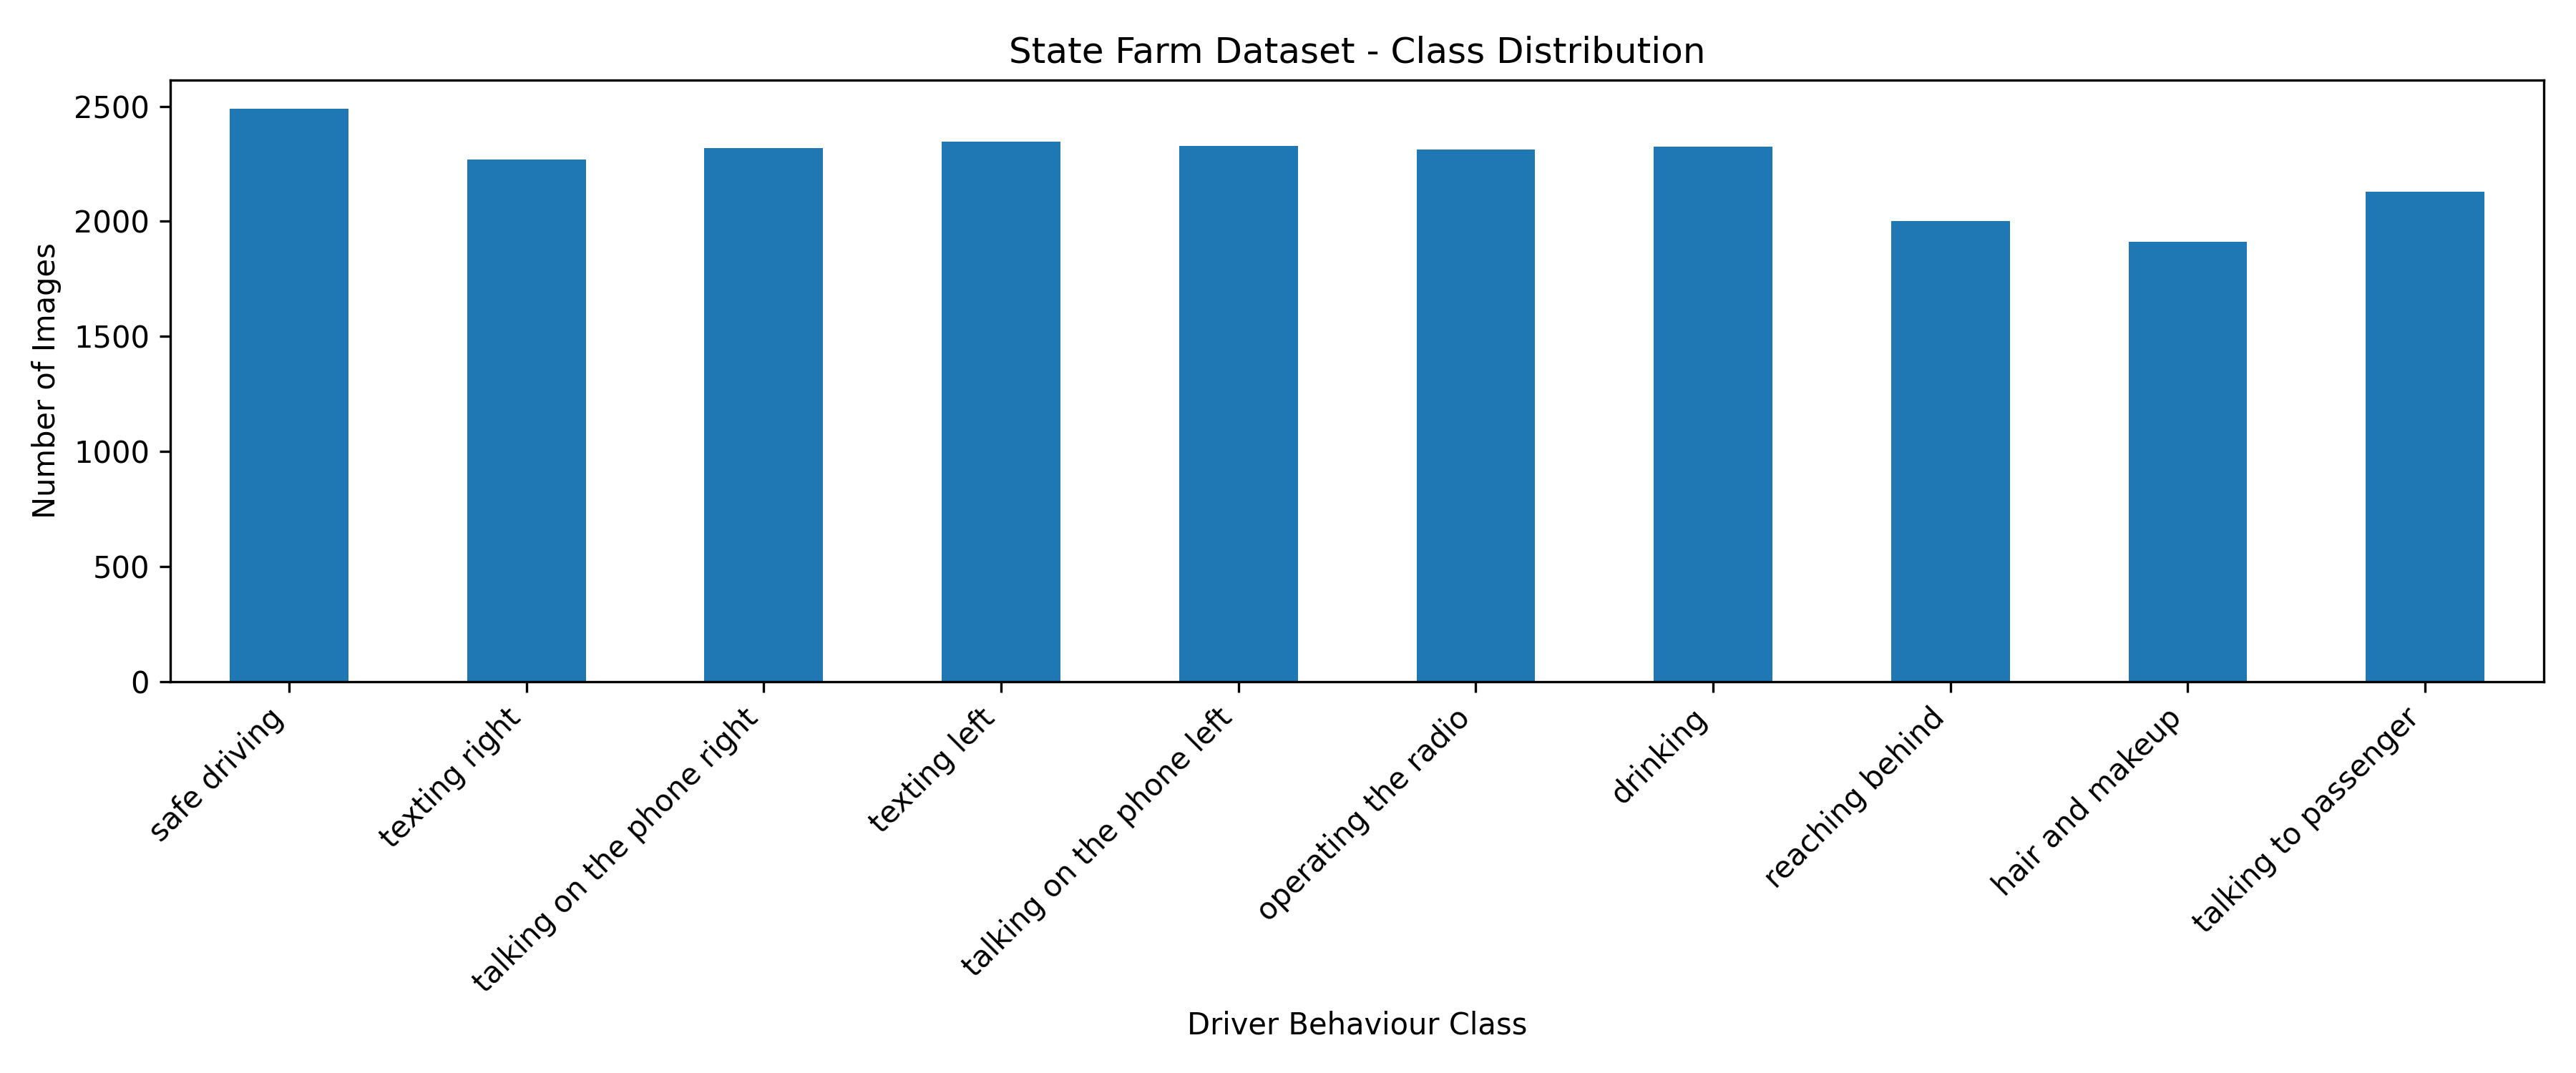
\includegraphics[width=\linewidth]{state_farm_class_distribution.png}
		\caption{Class distribution}
		\label{fig:app-sf-classes}
	\end{subfigure}
	\hfill
	\begin{subfigure}{0.99\textwidth}
		\centering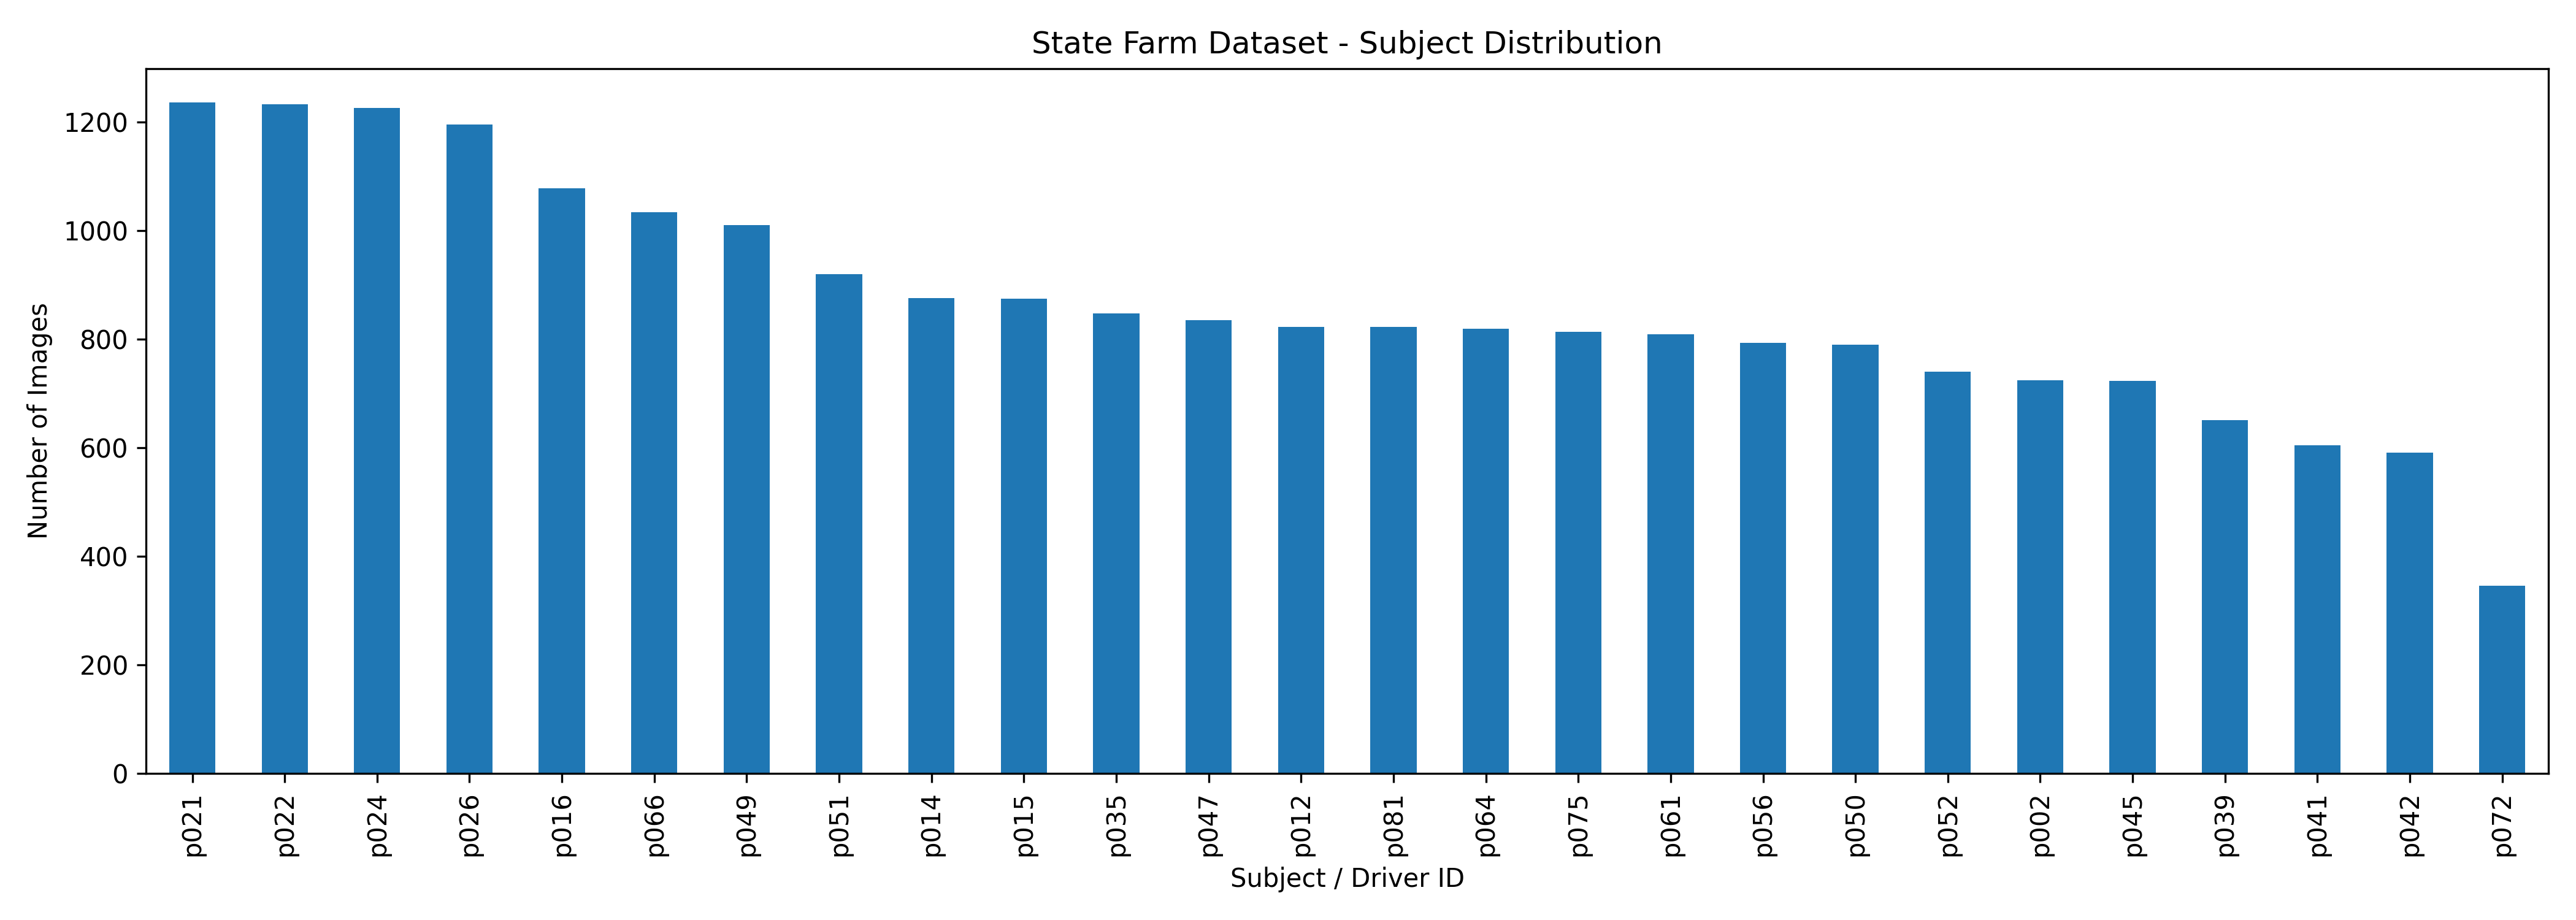
\includegraphics[width=\linewidth]{state_farm_subject_distribution.png}
		\caption{Images per driver}
		\label{fig:app-sf-subjects}
	\end{subfigure}
	\caption{State Farm dataset composition.}
	\label{fig:app-sf-composition}
\end{figure}

\chapter{Full Per-Class Classification Reports}
\label{app:classreports}

Supporting evidence for Sections~\ref{sec:qr-baseline}, \ref{sec:qr-crossview}, \ref{sec:qr-lowlight}, and ~\ref{sec:qr-class-errors} is provided. All figures are calculated based on the test partitions of held-out subjects from Appendix~\ref{app:splits}. 

\begin{table}[H]
\centering
\caption{Per-class F1 for the three single-view baseline models, State Farm test set.}
\label{tab:app-sf-f1}
\small
\begin{tabular}{lcccr}
\toprule
\textbf{Class} & \textbf{Baseline CNN} & \textbf{MobileNetV2} & \textbf{EfficientNet-B0} & \textbf{Support} \\
\midrule
c0 safe driving & 0.620 & 0.707 & 0.738 & 316 \\
c1 texting right & 0.747 & 0.788 & 0.888 & 325 \\
c2 phone right & 0.928 & 0.970 & 0.966 & 338 \\
c3 texting left & 0.901 & 0.974 & 0.971 & 322 \\
c4 phone left & 0.944 & 0.917 & 0.880 & 345 \\
c5 operating radio & 0.783 & 0.960 & 0.900 & 327 \\
c6 drinking & 0.884 & 0.872 & 0.817 & 311 \\
c7 reaching behind & 0.698 & 0.935 & 0.878 & 293 \\
c8 hair and makeup & 0.619 & 0.708 & 0.600 & 251 \\
c9 talking to passenger & 0.403 & 0.572 & 0.520 & 258 \\
\midrule
Macro average & 0.753 & \textbf{0.840} & 0.816 & 3{,}086 \\
Weighted average & 0.766 & \textbf{0.849} & 0.828 & 3{,}086 \\
\bottomrule
\end{tabular}
\end{table}

\begin{table}[H]
\centering
\caption{MobileNetV2 full per-class report, State Farm subject-wise test set (accuracy 84.67\%).}
\label{tab:app-mnv2}
\small
\begin{tabular}{lcccr}
\toprule
\textbf{Class} & \textbf{Precision} & \textbf{Recall} & \textbf{F1} & \textbf{Support} \\
\midrule
c0 safe driving & 0.664 & 0.756 & 0.707 & 316 \\
c1 texting right & 0.960 & 0.668 & 0.788 & 325 \\
c2 phone right & 0.985 & 0.956 & 0.970 & 338 \\
c3 texting left & 0.972 & 0.975 & 0.974 & 322 \\
c4 phone left & 0.926 & 0.907 & 0.917 & 345 \\
c5 operating radio & 1.000 & 0.924 & 0.960 & 327 \\
c6 drinking & 0.819 & 0.932 & 0.872 & 311 \\
c7 reaching behind & 0.971 & 0.901 & 0.935 & 293 \\
c8 hair and makeup & 0.631 & 0.805 & 0.708 & 251 \\
c9 talking to passenger & 0.567 & 0.578 & 0.572 & 258 \\
\midrule
Macro average & 0.849 & 0.840 & 0.840 & 3{,}086 \\
Weighted average & 0.861 & 0.847 & 0.849 & 3{,}086 \\
\bottomrule
\end{tabular}
\end{table}

\begin{table}[H]
\centering
\caption{Cross-view MobileNetV2, frozen-backbone against fine-tuned, mixed-view test set (17{,}992 images).}
\label{tab:app-crossview}
\footnotesize
\begin{tabular}{lrcccccc}
\toprule
& & \multicolumn{3}{c}{\textbf{Frozen-backbone} (75.94\%)} & \multicolumn{3}{c}{\textbf{Fine-tuned} (91.76\%)} \\
\cmidrule(lr){3-5}\cmidrule(lr){6-8}
\textbf{Class} & \textbf{Support} & \textbf{P} & \textbf{R} & \textbf{F1} & \textbf{P} & \textbf{R} & \textbf{F1} \\
\midrule
safe\_driving & 9{,}006 & 0.887 & 0.881 & 0.884 & 0.944 & 0.977 & 0.960 \\
texting\_right & 1{,}309 & 0.687 & 0.502 & 0.580 & 0.924 & 0.765 & 0.837 \\
phone\_right & 1{,}332 & 0.722 & 0.642 & 0.680 & 0.840 & 0.986 & 0.907 \\
texting\_left & 1{,}286 & 0.422 & 0.768 & 0.545 & 0.974 & 0.821 & 0.891 \\
phone\_left & 1{,}341 & 0.591 & 0.782 & 0.673 & 0.906 & 0.899 & 0.903 \\
adjusting\_radio & 327 & 0.928 & 0.746 & 0.827 & 0.974 & 0.927 & 0.950 \\
drinking & 1{,}273 & 0.754 & 0.610 & 0.675 & 0.840 & 0.833 & 0.837 \\
reaching\_behind & 835 & 0.884 & 0.695 & 0.778 & 0.953 & 0.884 & 0.917 \\
hair\_or\_makeup & 1{,}025 & 0.696 & 0.537 & 0.606 & 0.867 & 0.876 & 0.871 \\
talking\_to\_passenger & 258 & 0.614 & 0.136 & 0.222 & 0.604 & 0.519 & 0.558 \\
\midrule
Macro average & 17{,}992 & 0.719 & 0.630 & 0.647 & 0.883 & 0.849 & 0.863 \\
Weighted average & 17{,}992 & 0.781 & 0.759 & 0.761 & 0.918 & 0.918 & 0.916 \\
\bottomrule
\end{tabular}
\end{table}

\begin{table}[H]
\centering
\caption{Lighting stage: day-only baseline (night-only test set, 1{,}500 images), frozen-backbone and fine-tuned (merged day+night test set, 4{,}586 images). The baseline's zero-recall rows are the collapse described in Section~\ref{sec:qr-lowlight}.}
\label{tab:app-lowlight}
\footnotesize
\begin{tabular}{lcccccccc}
\toprule
& \multicolumn{2}{c}{\textbf{Baseline} (19.53\%)} & \multicolumn{3}{c}{\textbf{Frozen} (62.30\%)} & \multicolumn{3}{c}{\textbf{Fine-tuned} (77.91\%)} \\
\cmidrule(lr){2-3}\cmidrule(lr){4-6}\cmidrule(lr){7-9}
\textbf{Class} & \textbf{P} & \textbf{R} & \textbf{P} & \textbf{R} & \textbf{F1} & \textbf{P} & \textbf{R} & \textbf{F1} \\
\midrule
safe\_driving & 0.000 & 0.000 & 0.559 & 0.712 & 0.626 & 0.551 & 0.845 & 0.667 \\
texting\_right & 0.000 & 0.000 & 0.721 & 0.451 & 0.554 & 0.986 & 0.459 & 0.626 \\
phone\_right & 0.000 & 0.000 & 0.689 & 0.598 & 0.640 & 0.900 & 0.883 & 0.891 \\
texting\_left & 0.170 & 0.993 & 0.720 & 0.676 & 0.697 & 0.965 & 0.648 & 0.776 \\
phone\_left & 0.000 & 0.000 & 0.780 & 0.523 & 0.626 & 0.926 & 0.653 & 0.765 \\
adjusting\_radio & 0.000 & 0.000 & 0.732 & 0.851 & 0.787 & 0.998 & 0.960 & 0.979 \\
drinking & 0.000 & 0.000 & 0.392 & 0.764 & 0.518 & 0.638 & 0.889 & 0.743 \\
reaching\_behind & 0.233 & 0.960 & 0.784 & 0.858 & 0.819 & 0.880 & 0.975 & 0.925 \\
hair\_or\_makeup & 0.000 & 0.000 & 0.423 & 0.414 & 0.419 & 0.596 & 0.663 & 0.628 \\
talking\_to\_passenger & 0.000 & 0.000 & 0.820 & 0.336 & 0.477 & 0.719 & 0.821 & 0.767 \\
\midrule
Macro average & 0.040 & 0.195 & 0.662 & 0.618 & 0.616 & 0.816 & 0.780 & 0.777 \\
Weighted average & 0.040 & 0.195 & 0.664 & 0.623 & 0.621 & 0.822 & 0.779 & 0.779 \\
\bottomrule
\end{tabular}
\end{table}

\chapter{Quantisation Raw Figures}
\label{app:quant}

Supporting evidence for Section~\ref{sec:qr-quantisation} and Table~\ref{tab:consolidated} is provided. Exact file sizes have been read from the filesystem. Megabytes are calculated in bytes divided by $1024^2$ as in project’s results tables.

\begin{table}[H]
\centering
\caption{Exact model artefact sizes.}
\label{tab:app-sizes}
\small
\begin{tabularx}{\textwidth}{Ylrr}
\toprule
\textbf{Artefact} & \textbf{Format} & \textbf{Bytes} & \textbf{MB} \\
\midrule
\texttt{best\_mobilenetv2\_crossview\_finetuned.keras} & Keras float32 & 21{,}791{,}872 & 20.78 \\
\texttt{mobilenetv2\_crossview\_finetuned\_int8.tflite} & TFLite INT8 & 2{,}723{,}448 & 2.60 \\
\texttt{mobilenetv2\_crossview\_int8.tflite} & TFLite INT8 & 2{,}721{,}672 & 2.60 \\
\texttt{mobilenetv2\_crossview\_dynamicrange.tflite} & TFLite dynamic range & 2{,}518{,}480 & 2.40 \\
\midrule
\multicolumn{2}{l}{Compression ratio, float32 to INT8} & \multicolumn{2}{r}{\textbf{8.00$\times$}} \\
\bottomrule
\end{tabularx}
\end{table}

\begin{table}[H]
\centering
\caption{Quantisation before/after measurements. All samples are drawn from held-out subject-wise test partitions.}
\label{tab:app-quant}
\small
\begin{tabularx}{\textwidth}{YllccY}
\toprule
\textbf{Model} & \textbf{Sample} & \textbf{$n$} & \textbf{Float32} & \textbf{INT8} & \textbf{Agreement} \\
\midrule
Cross-view frozen & mixed front+side & 500 & 76.80\% & 76.00\% & 91.2\% \\
Cross-view frozen & random \texttt{side} & 300 & 59.30\% & 54.70\% & --- \\
Cross-view fine-tuned & random \texttt{side} & 300 & 80.00\% & 77.30\% & --- \\
Cross-view fine-tuned & held-out sample & 100 & \multicolumn{2}{c}{Keras vs. TFLite} & 100/100 \\
Cross-view fine-tuned & held-out sample & 100 & \multicolumn{2}{c}{board vs. laptop} & 100/100 \\
\bottomrule
\end{tabularx}
\end{table}

The two rows of board-versus-laptop agreement illustrate the measurements proving the numerical correctness of from-source ARM32 runtime (Section~\ref{sec:qr-runtime-correctness}). Dynamic-range variant was created and validated but not deployed since the INT8 variant was used in the accuracy evaluation.

\chapter{FPGA Synthesis Report Excerpts}
\label{app:fpga}

Supporting evidence for Section~\ref{sec:qr-fpga} is provided. The excerpts are taken verbatim from Vivado program created by Vivado 2017.4 targeting "7a35tcpg236-1" with the design status marked as “Synthesized” and provided out of context.

\begin{table}[H]
\centering
\caption{Slice logic utilisation (from \texttt{utilization.rpt}).}
\label{tab:app-util}
\small
\begin{tabular}{lrrr}
\toprule
\textbf{Site type} & \textbf{Used} & \textbf{Available} & \textbf{Util.\%} \\
\midrule
Slice LUTs & 18 & 20{,}800 & 0.09 \\
\quad LUT as logic & 18 & 20{,}800 & 0.09 \\
\quad LUT as memory & 0 & 9{,}600 & 0.00 \\
Slice registers & 13 & 41{,}600 & 0.03 \\
\quad Register as flip-flop & 13 & 41{,}600 & 0.03 \\
\quad Register as latch & 0 & 41{,}600 & 0.00 \\
F7 muxes & 0 & 16{,}300 & 0.00 \\
F8 muxes & 0 & 8{,}150 & 0.00 \\
Block RAM & 0 & --- & 0.00 \\
DSP slices & 0 & --- & 0.00 \\
\bottomrule
\end{tabular}
\end{table}

\begin{figure}[H]
\centering
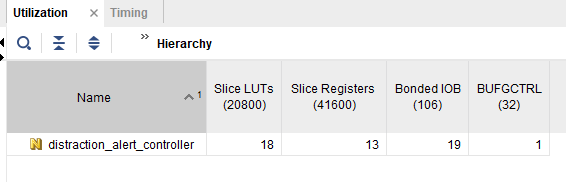
\includegraphics[width=0.8\textwidth]{vivado_utilization_report.png}
\caption{Vivado's own utilization report view for the synthesized alert controller, confirming the 18 LUTs / 13 registers reported in Table~\ref{tab:app-util}.}
\label{fig:vivado-util}
\end{figure}

All 13 registers are clock-enabled flip-flops with synchronous reset. Vivado’s report notes that “the final LUT count, after physical optimizations and full implementation, is typically lower,” hence the claim in Section~\ref{sec:qr-fpga} about 18 LUTs being conservative post-synthesis estimate rather than post-placement-and-routing.

\begin{table}[H]
\centering
\caption{Design timing summary, clock constrained at 100~MHz.}
\label{tab:app-timing}
\small
\begin{tabular}{lrr}
\toprule
\textbf{Metric} & \textbf{Value} & \textbf{Failing endpoints} \\
\midrule
Worst negative slack (WNS) & $+7.276$ ns & 0 of 17 \\
Total negative slack (TNS) & 0.000 ns & --- \\
Worst hold slack (WHS) & $+0.272$ ns & 0 of 17 \\
Total hold slack (THS) & 0.000 ns & --- \\
Worst pulse width slack (WPWS) & $+4.500$ ns & 0 of 13 \\
\bottomrule
\end{tabular}
\end{table}

\begin{figure}[H]
\centering
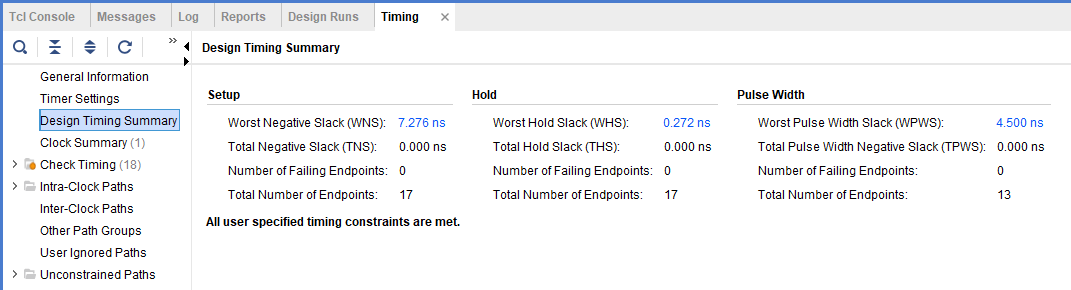
\includegraphics[width=0.99\textwidth]{vivado_timing_summary.png}
\caption{Vivado's timing summary panel, confirming the worst-negative-slack figure reported in Table~\ref{tab:app-timing}.}
\label{fig:vivado-timing}
\end{figure}


\chapter{Alert Delivery Path and Its Verification}
\label{app:alertpath}

Evidence in support of the alert-delivery pipeline is summarized in Chapter \ref{ch:methodology}. The board runs an endless capture-classify loop that uses hysteresis logic as a straight copy of "distraction\_alert\_controller.v" in Python. It uses the same 40\% confidence threshold, the same eight-tick set and clear counters, and follows the exact same process of incrementing the counters and checking set and clear ticks in relation to the increments; hence, a "low confidence" tick leaves both counters unaffected in the same way as the RTL always-block does. On the rising edge of an alert, and on that alone (and not once per classified frame), the system posts the class, confidence, and the JPEG-encoded triggering frame to the FastAPI backend. The backend saves the image and serves it to the Kotlin Android client via the same bearer token authentication as the rest of the API.

An end-to-end trigger would require keeping a distracted position in front of the camera for about seventy seconds due to the inference speed of the board. Consequently, validation was done in three independent layers.

\begin{table}[H]
\centering
\caption{Three-layer verification of the alert-delivery path.}
\label{tab:app-alertpath}
\small
\begin{tabularx}{\textwidth}{>{\raggedright\arraybackslash}p{2.6cm}YY}
\toprule
\textbf{Layer} & \textbf{What was exercised} & \textbf{Result} \\
\midrule
1. Logic equivalence & The Python hysteresis port replayed against the same five scenarios as the Verilog testbench (sustained safe, sub-threshold burst, sustained distraction, an uncertain tick mid-run, sustained safe again). & 10/10 checks passed, matching the testbench's expected transitions. \\
2. Hardware execution & Real webcam frames through the real INT8 model and the real hysteresis state machine, on the board, with no synthetic data. & Ran cleanly end to end at $\sim$9.1\,s per tick, no crash and no false alert. \\
3. Network delivery & The production posting function imported and called directly, then the stored record retrieved from the backend and viewed in the Android client. & HTTP 200; record and image confirmed present and byte-identical. \\
\bottomrule
\end{tabularx}
\end{table}

Layer 1 shows that the deployed decision logic behaves the same as the hardware design verified in Section~\ref{sec:qr-fpga}. Layer 2 shows that the full pipeline runs on real hardware. Layer 3 shows that the network call the loop actually makes reaches its destination. What the three layers together do not add up to is one single unattended physical demonstration. That limitation is stated here directly, not hidden.

\begin{figure}[H]
\centering
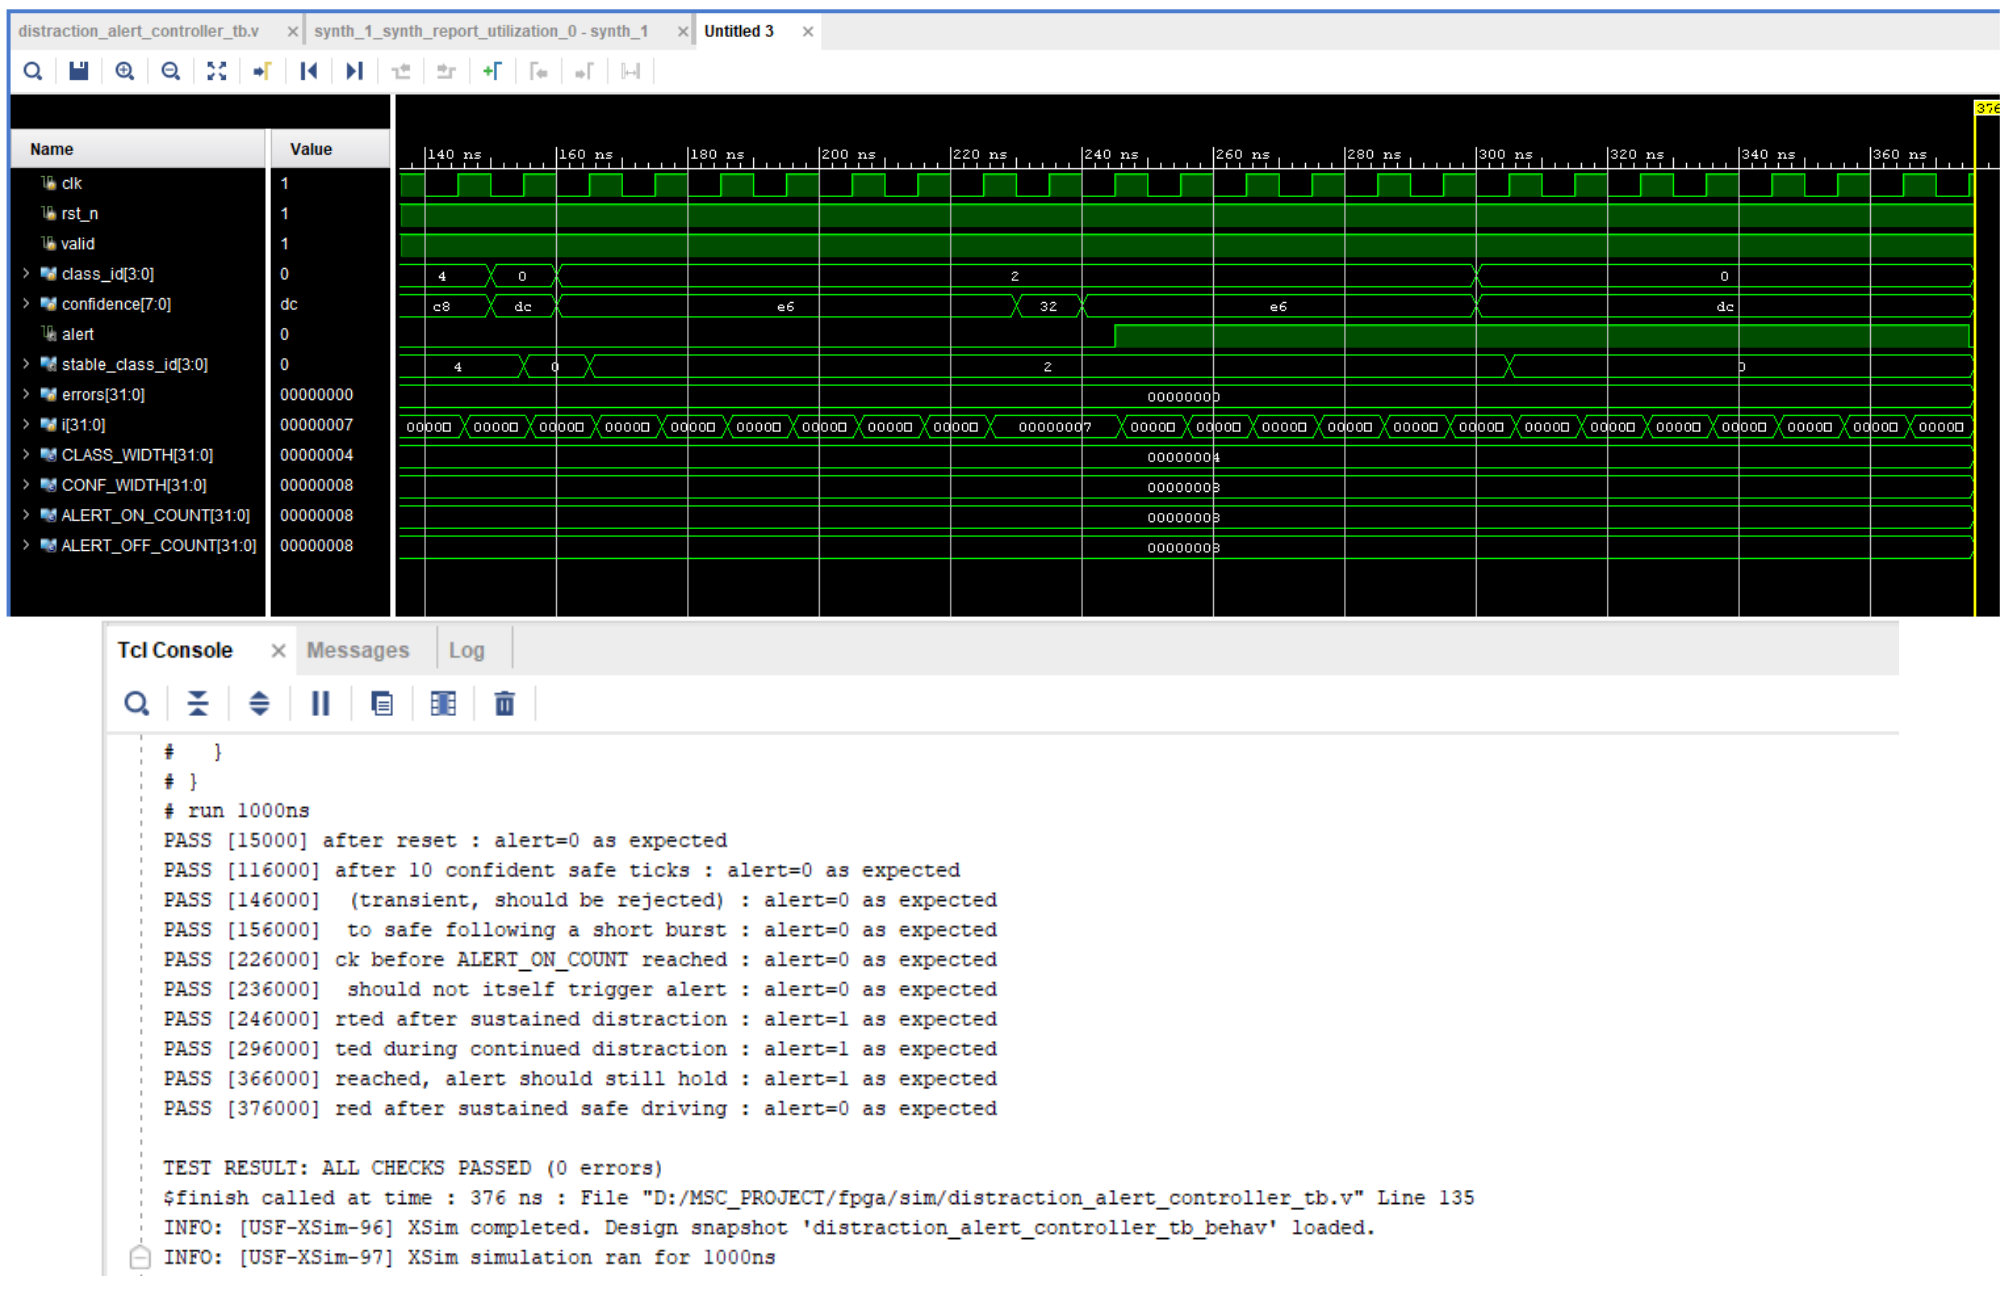
\includegraphics[width=0.99\textwidth]{vivado_testbench_sim.png}
\caption{The self-checking testbench run in Vivado's simulator: the waveform shows \texttt{alert} correctly staying low, then rising after sustained distraction and clearing after sustained safe driving, and the Tcl Console confirms all ten checks passed, matching Table~\ref{tab:app-alertpath} (Layer 1).}
\label{fig:testbench-sim}
\end{figure}

\begin{figure}[htbp]
\centering
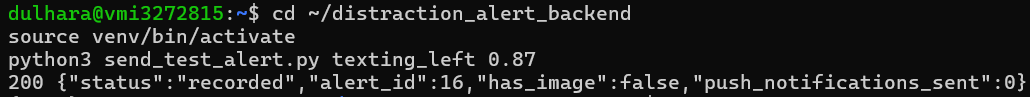
\includegraphics[width=0.75\textwidth]{backend_alert_received.png}\\[0.5em]
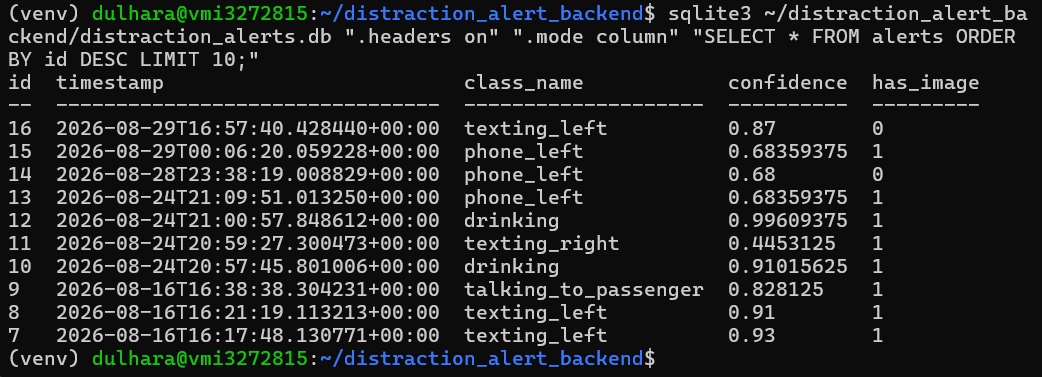
\includegraphics[width=0.75\textwidth]{backend_db_record.png}
\caption{The FastAPI backend receiving a real alert (top) and the same record persisted in its SQLite database (bottom), confirming the HTTP 200 and stored-record result reported in Table~\ref{tab:app-alertpath}.}
\label{fig:backend-alert}
\end{figure}


\begin{figure}[H]
\centering
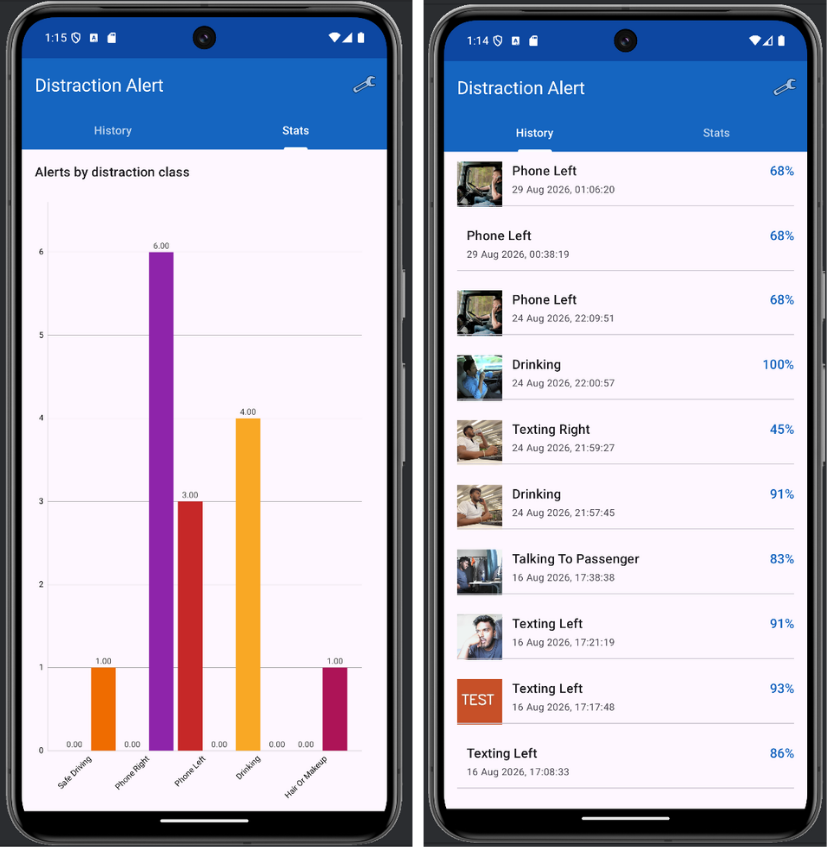
\includegraphics[width=0.85\textwidth]{android_app_alert.png}
\caption{A real alert received on the Android client, showing the triggering frame and timestamp posted by the board.}
\label{fig:app-alert}
\end{figure}



\chapter{Physical Buzzer Alert Output}
\label{app:buzzer}

Support of the buzzer paragraph in Chapter \ref{ch:methodology} is provided in this appendix. This appendix covers why the board could not drive a buzzer at all before this work, what was built to fix that, the real problems hit along the way, and how the buzzer itself was diagnosed and driven correctly.

\section{The board could not control the header pin at all}

The available buzzer is a real two-pin passive one, having no transistor or driver circuit at all, and therefore requires a direct connection to a GPIO header pin. Inspecting "/sys/class/gpio" of the board's stock PYNQ image, only a single GPIO controller is found there, "zynq\_gpio", with none of those going to the board's PMOD headers. The PMOD and LED-related pins are on the FPGA-fabric I/O banks, not the processor's fixed MIO banks. Furthermore, there is no bitstream or overlay exposing those pins anywhere on the board's filesystem. Therefore, no part on the board can toggle a header pin from Python without a bitstream doing this job explicitly. This was determined directly and not through assumptions.

\section{The overlay}

A minimal Vivado project was created from scratch targeting the real device on the board. Project's Basys3 target used in Section~\ref{sec:fpga-alert-design}). The block design (Figure~\ref{fig:buzzer-bd}) includes a Zynq7 Processing System block and a single-bit AXI GPIO block. The processing-system block does not reconfigured. Linux is already running from the SD card independently of this design. It is included so Vivado generates the AXI clock, reset and address decode connections allowing the running processor to address a peripheral that exists in the reconfigurable fabric. The output of the GPIO block was connected to package pin V7, marked by the board's user guide as pin 1 of header J62 named as "PMOD2". \citep{xilinx2019ug850}.

\RequiredFigure[1.0\textwidth]{zc702_buzzer_overlay_block_design.png}{The buzzer overlay's Vivado block design. A Zynq7 Processing System block provides AXI/clock/reset plumbing to the already-running processor. A single-bit AXI GPIO block is the only new circuit, exposed externally as \texttt{buzzer\_o} on package pin V7.}{fig:buzzer-bd}

Three concrete build errors were faced and solved via reading Vivado's output messages rather than guessing. A manual clock connection automation command failed because the connection of the clock via AXI4 connection automation had already been done. After synthesis, implementation, and bitstream generation had finished without errors. 

\begin{figure}[H]
\centering
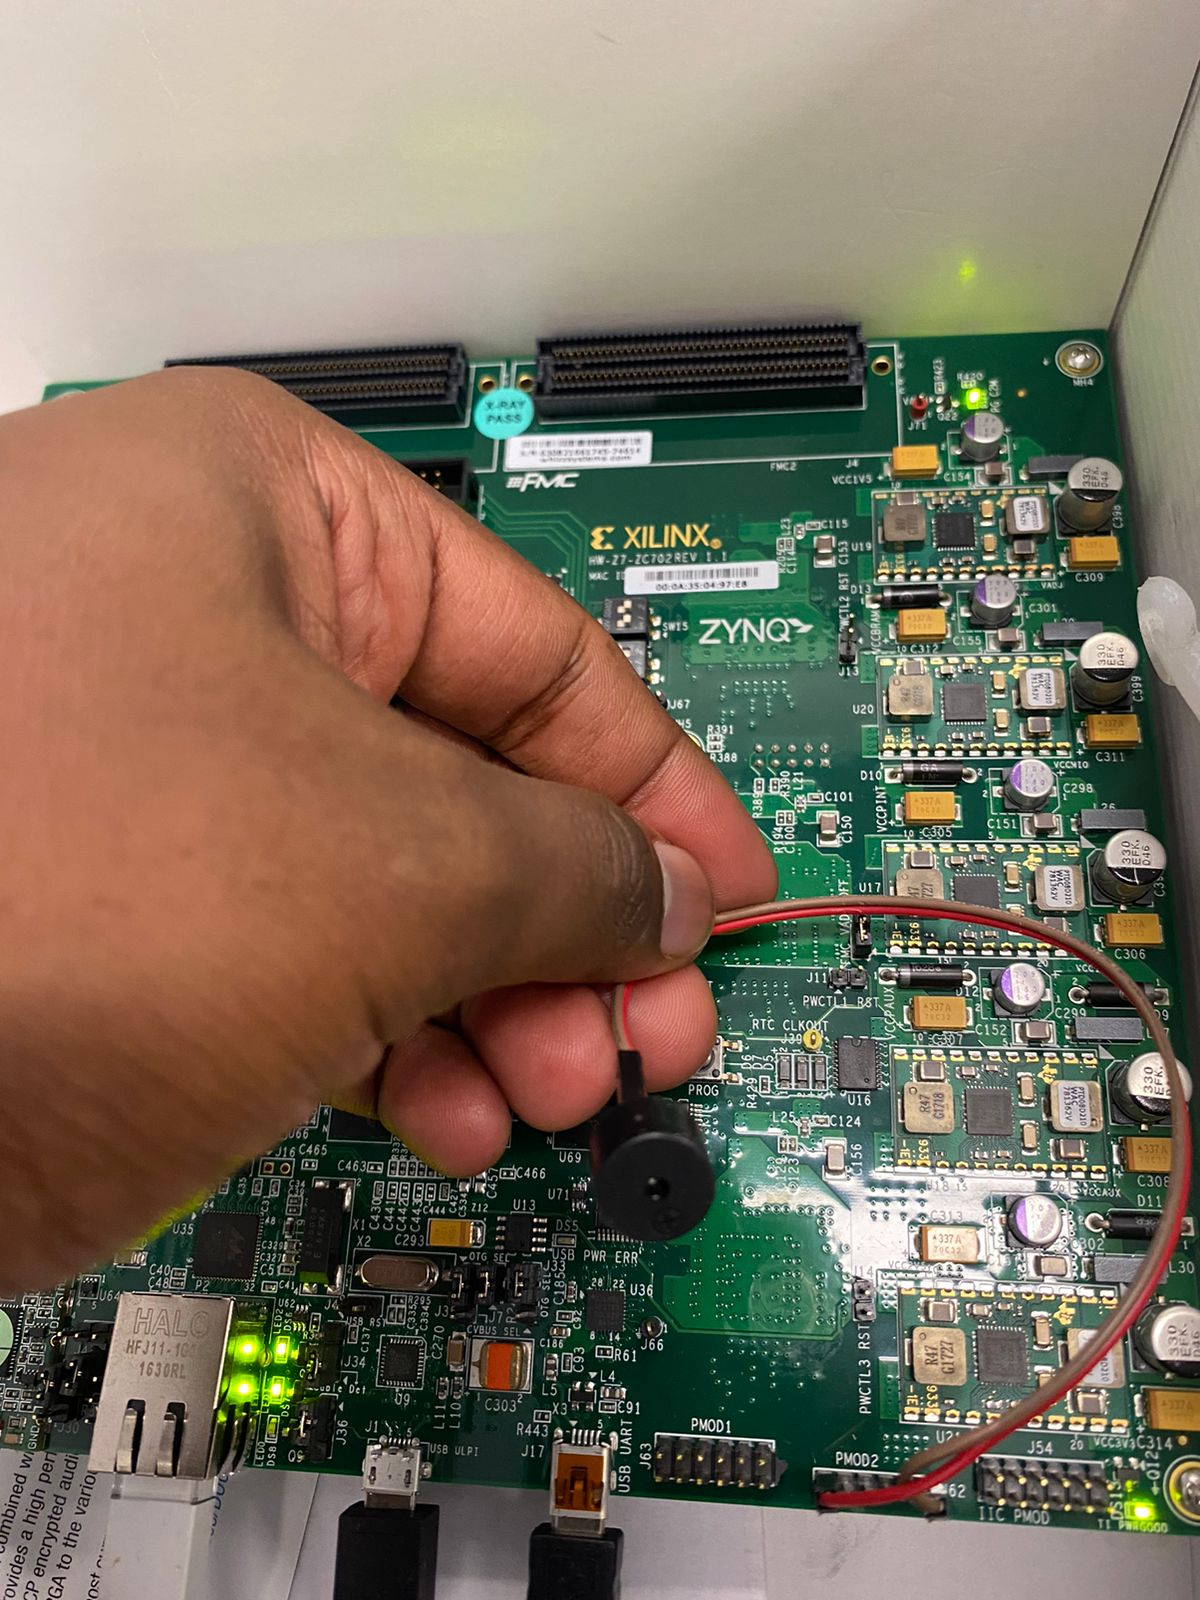
\includegraphics[width=0.65\textwidth]{zc702_buzzer_photo.jpg}
\caption{The ZC702 board with the passive buzzer wired directly to header pin J62 (PMOD2\_0), driven by the GPIO overlay described in this appendix.}
\label{fig:buzzer-photo}
\end{figure}


\section{Root permission and two unrelated Jupyter defects}

The loading of the hardware overlay failed because of a permission issue. Even though initially it seemed like a file permission issue, this was not the case. The software has an intrinsic requirement to be run with root privileges and will not work with another type of privileges regardless of file permissions. Initial attempts to solve the problem through file permissions modification were investigated and eventually proved ineffective because the check was about execution, not file access. The right solution was to configure the notebook service to start up with root privileges, which fixed the problem right away. Such configuration corresponds to the standard, expected one for boards of this kind; the specific board being tested had a different one. In the process of troubleshooting, two other minor problems were found and fixed. One setting secretly told the notebook service to use a wrong user-specific directory which made accessing a certain package impossible later when running tests on the device and the directory that the notebook browser displayed was different from the real one containing the notebooks, making them invisible.

\section{Driving a passive buzzer}

The first attempts to power the buzzer and keep it active failed with producing only a single click rather than a constant sound. This behavior is typical for such a simple buzzer that does not have an internal circuit to keep the sound going and emits it only while switching on and off and stays silent otherwise. Therefore, the solution was to rapidly switch the buzzer on and off in software using sufficient frequency to create a sound rather than clicks. Using a precisely controlled and constantly evaluated timer, rather than a plain built-in delay, led to the sound sounding more steady but at the price of taking up a full CPU core during the alert.

\section{Integration}

The hardware interface is created once, upon program initialization, rather than being reinitialized each time an alert is sent, since this would lead to considerable delay. The buzzer and the phone notification are triggered at the very same point in code, guaranteeing their synchronous triggering. This was checked by testing in the conditions of the actual system rather than using an easy shortcut test, since it relies on having administrator privileges which were ensured by fixing the problem described above.

\chapter{Selected Code Excerpts}
\label{app:code}

Supporting evidence for Sections~3.2.1, 3.4.1 and 3.5. The three excerpts below are the exact functions responsible for the subject-wise split, the quantisation-conversion fix and the FPGA decision logic. Full files are in project's GitHub repository

\section*{Subject-wise splitting}

\begin{lstlisting}[language=Python, caption={Subject-wise train/validation/test split.}, label=lst:subject-split]
from sklearn.model_selection import GroupShuffleSplit

SEED = 42

# First split: 70% train, 30% temporary set
gss1 = GroupShuffleSplit(n_splits=1, train_size=0.70, random_state=SEED)
train_idx, temp_idx = next(gss1.split(df, groups=df["subject"]))

train_df = df.iloc[train_idx].reset_index(drop=True)
temp_df = df.iloc[temp_idx].reset_index(drop=True)

# Second split: temporary set into validation and test
gss2 = GroupShuffleSplit(n_splits=1, train_size=0.50, random_state=SEED)
val_idx, test_idx = next(gss2.split(temp_df, groups=temp_df["subject"]))
\end{lstlisting}

\section*{The augmentation-layer conversion fix}

\begin{lstlisting}[language=Python, caption={Disabling the augmentation step so it isn't included when converting the model.}, label=lst:monkeypatch]
aug_layer = None
for layer in model.layers:
    if "augmentation" in layer.name.lower():
        aug_layer = layer
        break
if aug_layer is None:
    raise ValueError("Could not find augmentation layer.")

aug_layer.call = lambda inputs, training=None: inputs
print("Monkey-patched augmentation layer:", aug_layer.name)
\end{lstlisting}

\section*{FPGA alert-controller RTL}

\begin{lstlisting}[language=Verilog, caption={The alert-controller logic: only raises or clears an alert after eight confident readings in a row, so a single flickered guess can't trigger it.}, label=lst:verilog-controller]
`timescale 1ns / 1ps

module distraction_alert_controller #(
    parameter integer CLASS_WIDTH     = 4,
    parameter integer CONF_WIDTH      = 8,
    parameter integer CNT_WIDTH       = 4,
    parameter [CLASS_WIDTH-1:0] SAFE_CLASS     = 4'd0,
    parameter [CONF_WIDTH-1:0]  CONF_THRESHOLD = 8'd102,
    parameter integer ALERT_ON_COUNT  = 8,
    parameter integer ALERT_OFF_COUNT = 8
)(
    input  wire                     clk,
    input  wire                     rst_n,
    input  wire                     valid,
    input  wire [CLASS_WIDTH-1:0]   class_id,
    input  wire [CONF_WIDTH-1:0]    confidence,
    output reg                      alert,
    output reg  [CLASS_WIDTH-1:0]   stable_class_id
);
    reg [CNT_WIDTH-1:0] distracted_run;
    reg [CNT_WIDTH-1:0] safe_run;
    wire is_distracted = valid && (class_id != SAFE_CLASS) && (confidence >= CONF_THRESHOLD);
    wire is_safe       = valid && (class_id == SAFE_CLASS) && (confidence >= CONF_THRESHOLD);
    always @(posedge clk) begin
        if (!rst_n) begin
            alert           <= 1'b0;
            stable_class_id <= SAFE_CLASS;
            distracted_run  <= {CNT_WIDTH{1'b0}};
            safe_run        <= {CNT_WIDTH{1'b0}};
        end else begin
            if (valid)
                stable_class_id <= class_id;
            if (is_distracted) begin
                if (distracted_run < ALERT_ON_COUNT[CNT_WIDTH-1:0])
                    distracted_run <= distracted_run + 1'b1;
                safe_run <= {CNT_WIDTH{1'b0}};
            end else if (is_safe) begin
                if (safe_run < ALERT_OFF_COUNT[CNT_WIDTH-1:0])
                    safe_run <= safe_run + 1'b1;
                distracted_run <= {CNT_WIDTH{1'b0}};
            end
            if (!alert && is_distracted && (distracted_run >= (ALERT_ON_COUNT[CNT_WIDTH-1:0] - 1'b1)))
                alert <= 1'b1;
            else if (alert && is_safe && (safe_run >= (ALERT_OFF_COUNT[CNT_WIDTH-1:0] - 1'b1)))
                alert <= 1'b0;
        end
    end
endmodule
\end{lstlisting}


\chapter{Repository and Notebook Map}
\label{app:repo}

The project is also published as a working repository on GitHub, where the same code, notebooks and results shown throughout this report can be browsed and downloaded directly, at \url{https://github.com/LangaXD/FPGA-Based-Driver-Distraction-Detection-System-Using-Image-Classification}.

\RequiredFigure[0.9\textwidth]{github_repo.png}{The project's GitHub repository.}{fig:github-repo}





\end{document}